\documentclass[usenames,dvipsnames,notheorems]{beamer}

\usefonttheme[onlymath]{serif}

% silence annoying warnings
\usepackage{silence}
\usepackage{caption}
\WarningFilter{remreset}{The remreset package}
\usepackage{xcolor}
%\usepackage{algorithm}
%\usepackage{algorithmic}
\usepackage{centernot}
\usepackage{dsfont}
\usepackage[ruled, vlined]{algorithm2e} % algorithm environments

\def\numSlides{32}

%% Math macros for LaTex Projects 
%% Maintainer: Aaron Mishkin <amishkin@cs.stanford.edu>
%% Original Source: Mark Schmidt (UBC CS), Ben Bloem-Reddy (UBC Stats).

%% Easy bold-face 

\def\bfA{\mathbf{A}}
\def\bfB{\mathbf{B}}
\def\bfC{\mathbf{C}}
\def\bfD{\mathbf{D}}
\def\bfE{\mathbf{E}}
\def\bfF{\mathbf{F}}
\def\bfG{\mathbf{G}}
\def\bfH{\mathbf{H}}
\def\bfI{\mathbf{I}}
\def\bfJ{\mathbf{J}}
\def\bfK{\mathbf{K}}
\def\bfL{\mathbf{L}}
\def\bfM{\mathbf{M}}
\def\bfN{\mathbf{N}}
\def\bfO{\mathbf{O}}
\def\bfP{\mathbf{P}}
\def\bfQ{\mathbf{Q}}
\def\bfR{\mathbf{R}}
\def\bfS{\mathbf{S}}
\def\bfT{\mathbf{T}}
\def\bfU{\mathbf{U}}
\def\bfV{\mathbf{V}}
\def\bfW{\mathbf{W}}
\def\bfX{\mathbf{X}}
\def\bfY{\mathbf{Y}}
\def\bfZ{\mathbf{Z}}

% bb series
\def\bbA{\mathbb{A}}
\def\bbB{\mathbb{B}}
\def\bbC{\mathbb{C}}
\def\bbD{\mathbb{D}}
\def\bbE{\mathbb{E}}
\def\bbF{\mathbb{F}}
\def\bbG{\mathbb{G}}
\def\bbH{\mathbb{H}}
\def\bbI{\mathbb{I}}
\def\bbJ{\mathbb{J}}
\def\bbK{\mathbb{K}}
\def\bbL{\mathbb{L}}
\def\bbM{\mathbb{M}}
\def\bbN{\mathbb{N}}
\def\bbO{\mathbb{O}}
\def\bbP{\mathbb{P}}
\def\bbQ{\mathbb{Q}}
\def\bbR{\mathbb{R}}
\def\bbS{\mathbb{S}}
\def\bbT{\mathbb{T}}
\def\bbU{\mathbb{U}}
\def\bbV{\mathbb{V}}
\def\bbW{\mathbb{W}}
\def\bbX{\mathbb{X}}
\def\bbY{\mathbb{Y}}
\def\bbZ{\mathbb{Z}}

% cal series
\def\calA{\mathcal{A}}
\def\calB{\mathcal{B}}
\def\calC{\mathcal{C}}
\def\calD{\mathcal{D}}
\def\calE{\mathcal{E}}
\def\calF{\mathcal{F}}
\def\calG{\mathcal{G}}
\def\calH{\mathcal{H}}
\def\calI{\mathcal{I}}
\def\calJ{\mathcal{J}}
\def\calK{\mathcal{K}}
\def\calL{\mathcal{L}}
\def\calM{\mathcal{M}}
\def\calN{\mathcal{N}}
\def\calO{\mathcal{O}}
\def\calP{\mathcal{P}}
\def\calQ{\mathcal{Q}}
\def\calR{\mathcal{R}}
\def\calS{\mathcal{S}}
\def\calT{\mathcal{T}}
\def\calU{\mathcal{U}}
\def\calV{\mathcal{V}}
\def\calW{\mathcal{W}}
\def\calX{\mathcal{X}}
\def\calY{\mathcal{Y}}
\def\calZ{\mathcal{Z}}

%% Theorem Environments %%
\usepackage{amsthm}
\usepackage{thmtools, thm-restate}

\declaretheorem[numberwithin=section]{theorem}
\declaretheorem[numberwithin=section]{proposition}
\declaretheorem[numberwithin=section]{lemma}
\declaretheorem[numberwithin=section]{definition}
\declaretheorem[numberwithin=section]{assumption}
\declaretheorem[numberwithin=section]{corollary}
\declaretheorem[numberwithin=section]{example}
\declaretheorem[numbered=no]{remark}

\makeatletter
\def\thm@space@setup{%
	\thm@preskip=1ex
	\thm@postskip=\thm@preskip % or whatever, if you don't want them to be equal
}
\makeatother

%% Floor and Ceiling %%
\usepackage{mathtools} % required for \DeclarePairedDelimeter

%% Stochastic Relations %% 

% almost sure:
\newcommand{\as}[1]{\stackrel{\text{\rm\tiny a.s.}}{#1}}
% a.s.\ equality:
\newcommand{\equas}{\stackrel{\text{\rm\tiny a.s.}}{=}}

% in distribution:
\newcommand{\dist}[1]{\stackrel{\text{\rm\tiny dist}}{#1}}
% equality in distribution:
\newcommand{\equdist}{\stackrel{\text{\rm\tiny dist}}{=}}

% independent
\newcommand{\ind}[0]{\perp \!\!\! \perp }

%% Variance, Expectation, etc %%
\newcommand{\Var}[1]{\textbf{Var}\sbr{#1}}

% ceiling and floor
\DeclarePairedDelimiter{\ceil}{\lceil}{\rceil}
\DeclarePairedDelimiter{\floor}{\lfloor}{\rfloor}
\newcommand{\argdot}{{\,\vcenter{\hbox{\tiny$\bullet$}}\,}} %generic argument dot

% absolute value
\newcommand{\abs}[1]{\left\vert #1\right\vert}

\newcommand{\seq}[1]{\rbr{#1}}

% easy bracketing:
\newcommand{\rbr}[1]{\left(#1\right)}
\newcommand{\sbr}[1]{\left[#1\right]}
\newcommand{\cbr}[1]{\left\{#1\right\}}
\newcommand{\abr}[1]{\left\langle#1\right\rangle}

% Norms
\def\norm#1{\|#1\|}
\def\biggnorm#1{\bigg\|#1\bigg\|}
% Random Variable Norms:
\def\psitwo#1{\|#1\|_{\psi_2}}
\def\psione#1{\|#1\|_{\psi_1}}

% mid
\newcommand{\biggmid}{\bigg \vert }

% argmax/argmin
\def\argmax{\mathop{\rm arg\,max}}
\def\argmin{\mathop{\rm arg\,min}}
\def\find{\mathop{\rm Find}}

% General Symbols
\def\half{\frac 1 2}
\newcommand{\inv}[1]{\frac{1}{#1}}
\newcommand{\halved}[1]{\frac{#1}{2}}
\newcommand{\R}{\mathbb{R}}
\newcommand{\eR}{\bar{\mathbb{R}}}

\newcommand{\into}{\rightarrow}

% Linear Algebra
\newcommand{\vspan}{\text{Span}}
\newcommand{\row}{\text{Row}}
\newcommand{\col}{\text{Col}}
\newcommand{\Null}{\text{Null}}
\newcommand{\Dim}{\text{Dim}}

% Functions
\newcommand{\dom}{\text{Dom}}
\newcommand{\sign}{\text{sign}}

% Gradient Descent Symbols
\newcommand{\oracle}{\mbox{\( \calO \)}}
\newcommand{\iter}{k}

\newcommand{\Lk}{L_{\zk}}
\newcommand{\Lmax}{L_{\text{max}}}
\newcommand{\mumax}{\mu_{\text{max}}}
\newcommand{\Lmin}{L_{\text{min}}}
\newcommand{\mumin}{\mu_{\text{min}}}

% iterates
\newcommand{\y}{y}
\newcommand{\yk}{y_k}
\newcommand{\ykk}{y_{k+1}}

\newcommand{\vk}{v_k}
\newcommand{\vkk}{v_{k+1}}

\newcommand{\w}{w}
\newcommand{\wk}{w_k}
\newcommand{\wkk}{w_{k+1}}
\newcommand{\wopt}{w^*}
\newcommand{\wbar}{\bar{w}}

\newcommand{\x}{x}
\newcommand{\xk}{x_k}
\newcommand{\xkplus}{x_k^+}
\newcommand{\xkk}{x_{k+1}}
\newcommand{\xopt}{x^*}
\newcommand{\xbar}{\xbar{w}}

% noise
\newcommand{\Z}{Z}
\newcommand{\z}{z}
\newcommand{\zk}{z_{k}}
\newcommand{\zkk}{z_{k+1}}
% step-sizes
\newcommand{\tetak}{{\tilde{\eta}}_{k}}
\newcommand{\etamin}{\eta_{\text{min}}}
\newcommand{\etamax}{\eta_{\text{max}}}
\newcommand{\etak}{\eta_k}
\newcommand{\etakk}{\eta_{k+1}}

\newcommand{\betak}{\beta_{k}}
\newcommand{\betakk}{\beta_{k+1}}
\newcommand{\alphak}{\alpha_{k}}
\newcommand{\alphakk}{\alpha_{k+1}}

\newcommand{\Ek}{\bbE_{\zk}}
\newcommand{\E}{\bbE}

% functions
\newcommand{\f}{f}
\newcommand{\fj}{f_i}
\newcommand{\fopt}{f^*}
% sub-sampled functions
\newcommand{\fk}{f_{i_k}}
\newcommand{\fkk}{f_{i_{(k+1)}}}
% gradients
\newcommand{\grad}{\nabla f}
% sub-sampled gradients
\newcommand{\gradk}{\nabla f_{i_k}}
\newcommand{\gradkk}{\nabla f_{i_{(k+1)}}}

%% Weak and strong growth constants
\newcommand{\sgc}{\rho}
\newcommand{\wgc}{\alpha}
%%%%%%%%%%%%%%%%%%%%%%%%%%%%%%%%%%%%%%%%%%%%%%%%%%%%%%%%%%

%% Etc %%  

%% add numbers to align* environments.
\newcommand{\addnumber}{\addtocounter{equation}{1}\tag{\theequation}}

%%%%%%%%%

\newcommand{\Wl}{W^{(l)}}
\newcommand{\Wll}{W^{(l+1)}}
\newcommand{\Wk}{W^{(L)}}

\newcommand{\Dl}{D^{(l)}}
\newcommand{\Dll}{D^{(l+1)}}
\newcommand{\Dk}{D^{(L)}}

\newcommand{\calDl}{\calD^{(l)}}
\newcommand{\calDll}{\calD^{(l+1)}}
\newcommand{\calDk}{\calD^{(L)}}

\newcommand{\nscalD}{\leftindex_{\text{ns}}{\calD}}
\newcommand{\nscalDl}{\leftindex_{\text{ns}}{\calD}^{(l)}}
\newcommand{\nscalDll}{\leftindex_{\text{ns}}{\calD}^{(l+1)}}
\newcommand{\nscalDk}{\leftindex_{\text{ns}}{\calD}^{(L)}}

\newcommand{\calKl}{\calK^{(l)}}
\newcommand{\calKll}{\calK^{(l+1)}}
\newcommand{\calKk}{\calK^{(L)}}

\newcommand{\calGl}{\calG^{(l)}}
\newcommand{\calGll}{\calG^{(l+1)}}
\newcommand{\calGk}{\calG^{(L)}}

\newcommand{\calCl}{\calC^{(l)}}
\newcommand{\calCll}{\calC^{(l+1)}}
\newcommand{\calCk}{\calC^{(L)}}

\newcommand{\nscalC}{\leftindex_{\text{ns}}{\calC}}
\newcommand{\nscalCl}{\leftindex_{\text{ns}}{\calC}^{(l)}}
\newcommand{\nscalCll}{\leftindex_{\text{ns}}{\calC}^{(l+1)}}
\newcommand{\nscalCk}{\leftindex_{\text{ns}}{\calC}^{(L)}}

\newcommand{\calHl}{\calH^{(l)}}
\newcommand{\calHll}{\calH^{(l+1)}}
\newcommand{\calHk}{\calH^{(L)}}

\newcommand{\Xl}{X^{(l)}}
\newcommand{\Xll}{X^{(l+1)}}
\newcommand{\Xk}{X^{(L)}}

\newcommand{\tXl}{X^{(l)}_{\text{gated}}}
\newcommand{\tXll}{X^{(l+1)}_{\text{gated}}}
\newcommand{\tXk}{X^{(L)}_{\text{gated}}}
\newcommand{\nsX}{\leftindex_{\text{ns}}{X}}
\newcommand{\nsXl}{\leftindex_{\text{ns}}{X}^{(l)}}
\newcommand{\nsXll}{\leftindex_{\text{ns}}{X}^{(l+1)}}
\newcommand{\nsXk}{\leftindex_{\text{ns}}{X}^{(L)}}

\newcommand{\Zl}{Z^{(l)}}
\newcommand{\Zll}{Z^{(l+1)}}
\newcommand{\Zk}{Z^{(L)}}

\newcommand{\Tl}{T^{(l)}}
\newcommand{\Tll}{T^{(l+1)}}
\newcommand{\Tk}{T^{(L)}}
\newcommand{\Tkopt}{T^{(L)*}}
\newcommand{\Tkbar}{\bar{T}^{(L)}}

\newcommand{\nsT}{\leftindex_{\text{ns}}{T}}
\newcommand{\nsTl}{\leftindex_{\text{ns}}{T}^{(l)}}
\newcommand{\nsTll}{\leftindex_{\text{ns}}{T}^{(l+1)}}
\newcommand{\nsTk}{\leftindex_{\text{ns}}{T}^{(L)}}
\newcommand{\nsTkopt}{\leftindex_{\text{ns}}{T}^{(L)*}}

\newcommand{\Vl}{V^{(l)}}
\newcommand{\Vll}{V^{(l+1)}}
\newcommand{\Vk}{V^{(L)}}

\newcommand{\Ul}{U^{(l)}}
\newcommand{\Ull}{U^{(l+1)}}
\newcommand{\Uk}{U^{(L)}}

\newcommand{\Gnorm}{\calG_{\text{norm}}}
\newcommand{\Tnorm}{\calT_{\text{norm}}}

%% matrix operators
\newcommand{\diag}{\text{diag}}

%% Group Lasso %%
\newcommand{\bi}{{b_i}}
\newcommand{\wi}{w_\bi}
\newcommand{\bwi}{\bar{w}_\bi}
\newcommand{\vi}{v_\bi}
\newcommand{\ci}{c_\bi}
\newcommand{\zi}{z_\bi}
\newcommand{\Xbi}{X_\bi}
\newcommand{\act}{{\calA_{\lambda}}}
\newcommand{\inact}{{\calI_{\lambda}}}
\newcommand{\tran}{{\calT_{\lambda}}}
\newcommand{\equi}{{\calE_{\lambda}}}

\newcommand{\acts}{{\calA_{\lambda}^{*}}}
\newcommand{\trans}{{\calT_{\lambda}^{*}}}

\newcommand{\wa}{w_\act}
\newcommand{\was}{w_\acts}
\newcommand{\we}{w_\equi}
\newcommand{\va}{v_\act}
\newcommand{\vas}{v_\acts}
\newcommand{\ca}{c_\act}
\newcommand{\cas}{c_\acts}
\newcommand{\ve}{v_\equi}
\newcommand{\ce}{c_\equi}
\newcommand{\Xa}{X_\act}
\newcommand{\Xas}{X_\acts}
\newcommand{\Xe}{X_\equi}

\newcommand{\wmin}{w^*}
\newcommand{\solfn}{\calW^*}

\newcommand{\Row}{\text{Row}}
\newcommand{\Span}{\text{Span}}
\newcommand{\Range}{\text{Range}}
\newcommand{\Rank}{\text{Rank}}

\newcommand{\Di}{\calD_{\bi}}
\newcommand{\Si}{\calN_{\bi}}
\newcommand{\Dis}{\Di^{*}}
\newcommand{\Sis}{\Ni^{*}}
\newcommand{\Ds}{\calD^{*}_\lambda}
\newcommand{\Ss}{\calN^{*}_\lambda}

\newcommand{\Ki}{K_{\bi}}
\newcommand{\Kid}{K_{\Di}}
\newcommand{\Kids}{K_{\Di^*}}
\newcommand{\Kd}{K_{\calD}}
\newcommand{\Kda}{K_{\calD \cap \act}}
\newcommand{\Kdas}{K_{\Gs}}
\newcommand{\Ka}{K_\act}

\newcommand{\Gs}{\calG^{*}_{\lambda}}

% dual parameters
\newcommand{\ri}{\rho_{\bi}}
\newcommand{\ract}{\rho_{\act}}
\newcommand{\racts}{\rho_{\acts}}
\newcommand{\rid}{\rho_{\Di}}
\newcommand{\rd}{\rho_{\calD}}
\newcommand{\rda}{\rho_{\calD \cap \act}}
\newcommand{\rdas}{\rho_{\Gs}}
\newcommand{\ra}{\rho_{\act}}
\newcommand{\rmin}{\rho^*}

\newcommand{\vmin}{v^*}
\newcommand{\nnz}{\text{nnz}}

% truncated parameters
\newcommand{\thetal}{\theta^{(l)}}

%% Plotting macros for LaTex Projects 
%% Maintainer: Aaron Mishkin <amishkin@cs.stanford.edu>


%% Tikz and PGFplots packages
\usepackage{tikz}
\usepackage{pgfplots}

% tikz and PGFplots libraries
\usepgfplotslibrary{fillbetween}
\usetikzlibrary{patterns}



%% tikz settings 
\tikzset{
    font={\fontsize{12pt}{12}\selectfont},
}

%% PGFplots settings 
\pgfplotsset{
    % version compatibility
    compat=1.5.1,
    % basic line-styles
    primary/.style={color=black, style=solid, line width=1.5pt}, 
    secondary/.style={color=red, style=solid, line width=1.5pt}, 
}


\usepackage{simplebeam}
\usetheme{simplebeamer}

\usetikzlibrary{shapes, arrows}
\usetikzlibrary{decorations.pathreplacing, calligraphy}

% node styles
\tikzstyle{Input}=[minimum size=0.5cm, fill=none, line width = 0.5mm, draw=black, shape=circle, text=black]
\tikzstyle{Hidden}=[minimum size=0.4cm, fill=blue, line width = 0.5mm, draw=blue, shape=circle, text=black]
\tikzstyle{Splits}=[inner sep=0.03cm, minimum size=0.3cm, line width = 0.3mm, draw=blue, shape=circle, text=black]
\tikzstyle{Output}=[minimum size=0.3cm, fill=white, line width = 0.5mm, draw=black, shape=circle, text=black]

% Edge styles
\tikzstyle{arrow}=[line width = 0.5mm]

% bib resources

\addbibresource[]{refs.bib}

\title{Global Optimization of Deep Relu Networks Using Convex Reformulations}
\author{Aaron Mishkin \and Mert Pilanci}
\collaborators{
	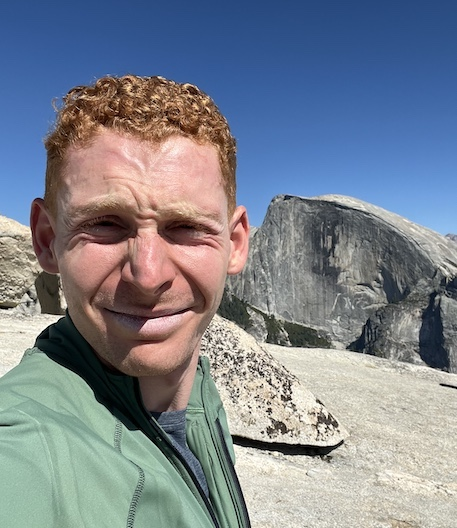
\includegraphics[width=0.3\linewidth]{assets/yosemite.jpeg}
	
\includegraphics[width=0.3\linewidth]{assets/mert.jpg}
}

\titlegraphic{
\includegraphics[width=0.4\textwidth]{assets/SUSig_2color_Stree_Left.eps}}

\newcommand{\horizontalrule}{
	{
			\vspace{-0.5em}
			\center \rule{\textwidth}{0.1em}
			\vspace{-0.2em}
		}
}

\newcommand{\red}[1]{\textcolor{Red}{#1}}
\newcommand{\green}[1]{\textcolor{ForestGreen}{#1}}
\newcommand{\blue}[1]{\textcolor{DarkBlue}{#1}}
\newcommand{\purple}[1]{\textcolor{Magenta}{#1}}

\definecolor{bad}{HTML}{eb6223}
\definecolor{good}{HTML}{9434ed}

\newcommand{\bad}[1]{\textcolor{bad}{#1}}
\newcommand{\good}[1]{\textcolor{good}{#1}}

\definecolor{sanddune}{rgb}{0.59, 0.44, 0.09}
\definecolor{byzantine}{rgb}{0.59, 0.44, 0.09}
\definecolor{ultramarine}{rgb}{0.07, 0.04, 0.56}
\definecolor{brightpink}{rgb}{1.0, 0.0, 0.5}

% toggle plotting tikz
\def\showtikz{}

%\logo{
\includegraphics[height=0.5cm]{assets/Block_S_2_color.eps}}

%\institute{Stanford University}
\frenchspacing
\date{}

\begin{document}

\maketitle
%% main content starts %%

\setbeamercolor{background canvas}{bg=LightCyan}

\begin{frame}{}
    \begin{center}
        \huge 1. Motivation: Global Optimization for Neural Networks
    \end{center}
\end{frame}
\setbeamercolor{background canvas}{bg=white}

\begin{frame}{Motivation: What is Global Optimization?}

    \begin{center}
        \large
        \textbf{Q}: What does global optimization mean for neural networks?
    \end{center}

    \pause
    \horizontalrule

    \textbf{Setup}:

    \vspace{0.5ex}
    \pause

    \begin{itemize}
        \item Let \( X \in \R^{n \times d} \) and \( y \in \R^{n \times c} \)
              be a \good{training set}.
              \pause
              \vspace{1ex}

        \item Fix an \good{architecture} \( \Delta \), \good{loss function} \( \calL \), and
              \good{regularizer} \( R \).
              \pause
              \vspace{1ex}

        \item Let \( f_\theta \) be the \good{neural network} parameterized by
              \( \theta \in \Delta \).
    \end{itemize}

    \pause
    \vspace{-0.5ex}

    \[
        \textbf{Global Opt.:} \, \, \theta^* \in
        \argmin_{\theta \in \Delta} \calL(f_\theta(X), y) + R(\theta).
    \]
    \pause

    \vspace{-3.5ex}

    \begin{center}
        %! TEX root = ../../main.tex
%% Illustration of step-sizes bound from Armijo line-search. 

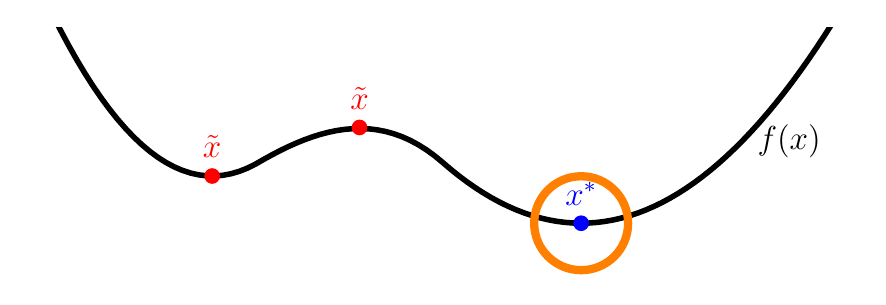
\begin{tikzpicture}[scale=1,
		declare function={
				objective(\x)=      (\x<=-1) * (2*\x*\x + 6*\x + 4)    +
				and(\x>-1, \x<=1) * (\x + 5 - pow(\x,3) - 5*\x*\x) / 4 +
				(\x>1) * (\x*\x - 5*\x + 4);
			}
	]
	\begin{axis}[
			width=\textwidth,
			height=4.75cm,
			axis x line=none, axis y line=none,
			ymin=-4.25, ymax=5, ytick={-5,...,5}, ylabel=$y$,
			xmin=-3.5, xmax=5.5, xtick={-5,...,7}, xlabel=$x$,
		]

		\addplot[name path=function, domain=-3.5:5.23, samples=100, line width=2pt]{objective(x)};

        \node[label={[text=blue]90:$x^*$},circle,fill=blue,inner sep=2pt] at (axis cs:2.5,-2.25) {};
        \node[label={[text=red]90:$\tilde x$},circle,fill=red,inner sep=2pt] at (axis cs:0.09717,1.3) {};
        \node[label={[text=red]90:$\tilde x$},circle,fill=red,inner sep=2pt] at (axis cs:-1.5,-0.5) {};

		\node[label={0:$f(x)$}] at (axis cs:4.2,0.8) {};
        \node<8->[circle,draw=orange,line width=3pt,fill=none,inner sep=12pt] at (axis cs:2.5,-2.25) {};
	\end{axis}
\end{tikzpicture}


    \end{center}

\end{frame}

\begin{frame}{Motivation: Why Bother?}

    \begin{center}
        \large
        \textbf{Q}: Why should we bother with global optimization?

        \pause
        \vspace{2ex}
        {\normalsize \good{(Stop and put on your machine learning hat)}}
    \end{center}

    \pause
    \horizontalrule

    \textbf{Problems}:

    \pause
    \vspace{0.5ex}

    \begin{itemize}
        \item \( f_\theta \) is highly \bad{non-linear}, usually
              \bad{non-smooth}, and the training problem is \bad{non-convex}.

              \pause
              \vspace{1ex}
              \begin{itemize}
                  \item[$\quad \longrightarrow$ ] Computing \( \theta^* \) is \bad{NP-Hard}
                        even when \( d \) is fixed \citep{froese2023hard}.
              \end{itemize}

              \pause
              \vspace{1ex}

        \item Local optimization methods like SGD and Adam are \good{simple},
              \good{fast}, and return ``\good{good enough}''
              solutions.
              \pause
              \vspace{1ex}

              \begin{itemize}
                  \item[$\quad \longrightarrow$ ] It's hard to argue against
                        successes like \good{ChatGPT} and \good{Claude}!
              \end{itemize}
    \end{itemize}

\end{frame}

\begin{frame}{Motivation: Image Generation using DALL$\cdot$E}

    \begin{center}
        \textit{A bowl of soup that is a portal to another
            dimension as digital art.}
    \end{center}
    \pause

    \begin{figure}[]
        \centering
        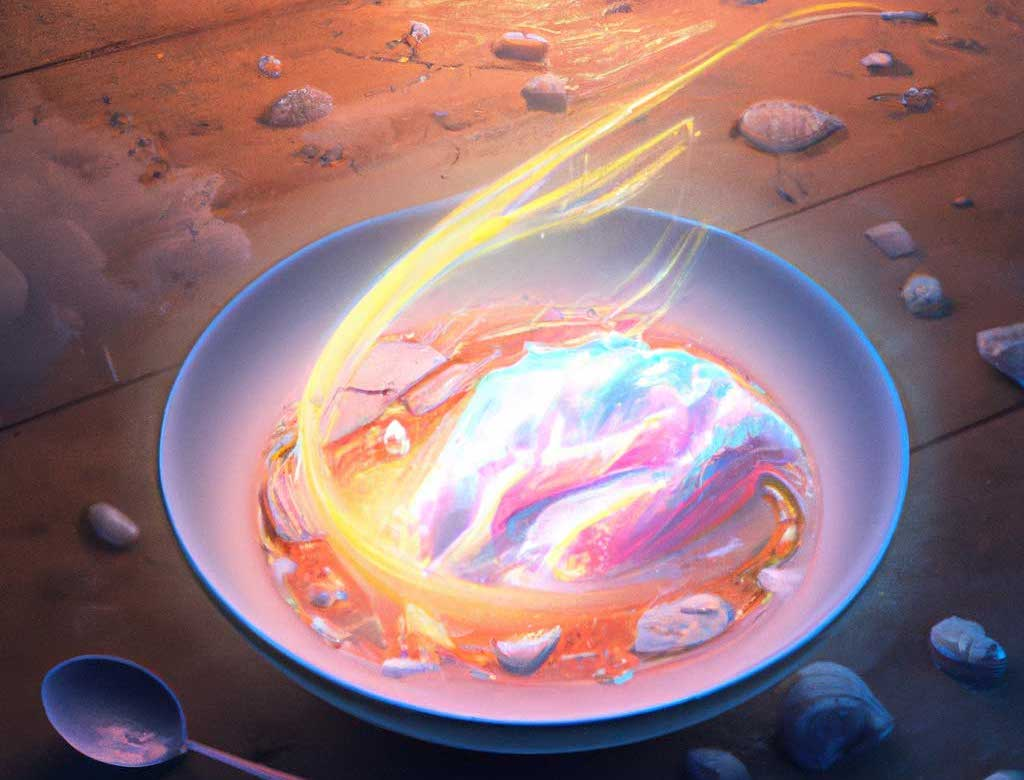
\includegraphics[width=0.55\linewidth]{assets/bowl_of_soup.jpg}
        \caption*{Generated by DALL$\cdot$E 2}%
    \end{figure}

    \pause

    \begin{center}
        DALL$\cdot$E 2 has 5.5 billion parameters and took \red{billions}
        of iterations to fit using Adam \citep{ramesh2022dalle}.
    \end{center}

    \source{https://openai.com/dall-e-2/}

\end{frame}

\begin{frame}{Motivation: Cost of Training}

    \begin{center}
        \large
        But this is small compared to recent LLMs!
    \end{center}

    \pause
    \horizontalrule

    Consider OpenAI's \good{GPT-4 model}:
    \vspace{1ex}
    \pause

    \begin{itemize}
        \item GPT-4 has \bad{\( 1.8 \) trillion} parameters;
              \vspace{0.5ex}
              \pause

        \item It was trained on \bad{\( \approx 13 \) trillion} tokens;
              \vspace{0.5ex}
              \pause

        \item Training used \bad{25,000 A100s} for 90 to 100 days;
              \vspace{0.5ex}
              \pause

        \item At \$1 per A100 hour, GPT-4 cost \bad{\( \approx \$63 \) million} dollars.
    \end{itemize}

    \source{https://the-decoder.com/gpt-4-architecture-datasets-costs-and-more-leaked/}

\end{frame}

\begin{frame}{Motivation: Training Artifacts}

    \textbf{Takeaway}:
    Modern deep learning models are \bad{huge} and \bad{extremely expensive}
    to train.
    \pause
    \vspace{1.0ex}

    \begin{itemize}
        \item But what is actually coming out of training?
              \pause
              \vspace{0.5ex}
        \item Let's ask ChatGPT!
    \end{itemize}

    \begin{figure}
        \centering
        \phantom{\includegraphics<-3>[width=0.9\textwidth]{assets/chat_gpt.png}}
        \includegraphics<4>[width=0.9\textwidth]{assets/chat_gpt.png}
        \includegraphics<5->[width=0.9\textwidth]{assets/chat_gpt_outlined.png}
    \end{figure}
\end{frame}

\begin{frame}{Motivation: Role of Global Optimization}

    Trained neural networks are identified \underline{mechanistically}:
    \vspace{1ex}
    \pause

    \begin{itemize}
        \item ``The model \( \theta \) is the result of training
              on \( (X, y) \) with
              \green{optimizer \( A \)} for
              \textcolor{brightpink}{\( b \) iterations} with
              \textcolor{ultramarine}{learning rate \( c \)}
              and\ldots''
              \vspace{1ex}
              \pause

        \item This goes beyond \bad{implicit regularization}:
              \( \theta \) cannot be disambiguated from the
              optimization routine!
    \end{itemize}

    \pause
    \horizontalrule

    \textbf{Q}: Why should we bother with global optimization?

    \vspace{1ex}
    \pause

    \begin{itemize}
        \item \( \theta^* \) has a \good{clear identity} and we
              can study it's behavior.
              \vspace{1ex}
              \pause

        \item We hope that \( \theta^* \) \good{generalizes better}.

              \vspace{1ex}
              \pause

        \item If not, at least we can \good{learn something}
              about the training problem and its solutions.
    \end{itemize}
\end{frame}

\begin{frame}{Motivation: Summary}

    \textbf{This Talk}: re-write training ReLU networks as a convex program.

    \pause
    \vspace{3ex}

    \textbf{Contributions}
    \begin{itemize}
        \item An \good{unconstrained convex reformulation} of fully-connected
              \( L \)-layer ReLU networks.
              \pause
              \vspace{1.5ex}

        \item \good{Polynomial time algorithms} for exactly fitting \( L \)-layer
              ReLU networks \underline{without biases}.

              \pause
              \vspace{1.5ex}

        \item \good{Polynomial-time approximations} for training \( 2 \)-layer
              ReLU networks \underline{with regularization}.
    \end{itemize}

\end{frame}

\setbeamercolor{background canvas}{bg=LightCyan}
\begin{frame}{}
    \begin{center}
        \huge
        2. Background on Convex Reformulations
    \end{center}
\end{frame}
\setbeamercolor{background canvas}{bg=white}

\begin{frame}{Convex Reformulations: Flavor of Results}

    \textbf{Basic Idea}: We start with a \bad{non-convex} optimization problem
    and derive an equivalent \good{convex} program.

    \pause
    \vspace{2em}

    \textbf{Equivalent} means:
    \pause
    \vspace{0.5em}
    \begin{itemize}
        \item The global minima have the same values: \( p^* = q^* \)
              \vspace{1em}
              \pause
        \item We can map every global minimum \( u^* \) for one problem into
              a global minimum \( v^* \) of the other.
    \end{itemize}

\end{frame}

\begin{frame}{Convex Reformulations: Two-Layer ReLU Networks}

    {\large \bad{Non-Convex Problem} (NC-ReLU)}
    \[
        \min_{W^{(1)}, W^{(2)}} \underbrace{\half \norm{\sum_{j=1}^{m_1}
                (X W^{(1)}_{\cdot, j})_+ W^{(2)}_{j} - y}_2^2}_{\text{Squared Error}}
        + \underbrace{\lambda \sum_{j=1}^m \norm{W^{(1)}_{\cdot, j}}_2^2
            + \norm{W^{(2)}_{j}}_2^2}_{\text{Weight Decay}},
    \]
    where \( \rbr{z}_+ = \max\cbr{z, 0} \), \( X \in \R^{n \times d} \), and
    \( y \in \R^{n} \).
    \pause

    \begin{figure}[]
        \centering
        \ifdefined\showtikz
            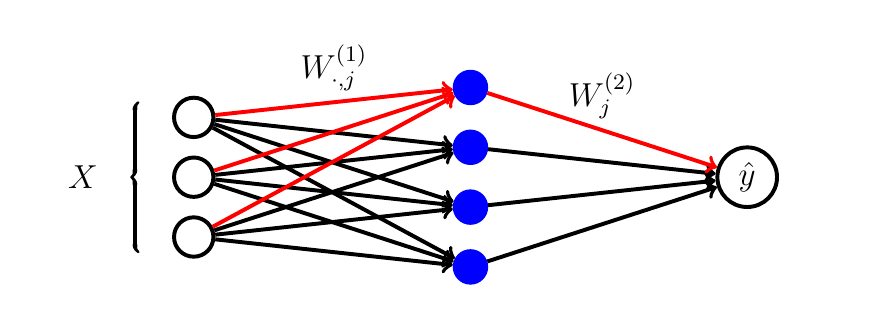
\begin{tikzpicture}[scale=1,
	]
	\begin{axis}[width=\linewidth, height=5cm,
			axis lines=none,  % don't print axis lines
			yticklabels={,,}, xticklabels={,,},
			ymin=0, ymax=9, y axis line style={-},
			xmin=0, xmax=15, x axis line style={-},
		]
		\node [] (input) at (axis cs:1,4) {$X$};
		\node [Input] (input1) at (axis cs:3,2) {};
		\node [Input] (input2) at (axis cs:3,4) {};
		\node [Input] (input3) at (axis cs:3,6) {};

		\draw [decorate, line width = 0.6mm,
			decoration = {calligraphic brace}] (axis cs:2,1.5) --  (axis cs:2,6.5);

		\node [Hidden] (hidden1) at (axis cs:8,1) {};
		\node [Hidden] (hidden2) at (axis cs:8,3) {};
		\node [Hidden] (hidden3) at (axis cs:8,5) {};
		\node [Hidden] (hidden4) at (axis cs:8,7) {};

		\draw [->, style=arrow, draw=black] (input1) -- (hidden1);
		\draw [->, style=arrow, draw=black] (input2) -- (hidden1);
		\draw [->, style=arrow, draw=black] (input3) -- (hidden1);

		\draw [->, style=arrow, draw=black] (input1) -- (hidden2);
		\draw [->, style=arrow, draw=black] (input2) -- (hidden2);
		\draw [->, style=arrow, draw=black] (input3) -- (hidden2);

		\draw [->, style=arrow, draw=black] (input1) -- (hidden3);
		\draw [->, style=arrow, draw=black] (input2) -- (hidden3);
		\draw [->, style=arrow, draw=black] (input3) -- (hidden3);

		\draw [->, style=arrow, draw=red] (input1) -- (hidden4);
		\draw [->, style=arrow, draw=red] (input2) -- (hidden4);
        \draw [->, style=arrow, draw=red] (input3) -- (hidden4) node[pos=0.5,above] {$W^{(1)}_{\cdot, j}$};

		\node [Output] (output) at (axis cs:13,4) {$\hat y$};

		\draw [->, style=arrow, draw=black] (hidden1) -- (output);
		\draw [->, style=arrow, draw=black] (hidden2) -- (output);
		\draw [->, style=arrow, draw=black] (hidden3) -- (output);
        \draw [->, style=arrow, draw=red] (hidden4) -- (output) node[pos=0.5,above] {$W^{(2)}_{j}$};
	\end{axis}

\end{tikzpicture}%

%\begin{tikzpicture}[scale=1,
%    ]
%    \begin{axis}[width=1.1\linewidth, height=5cm,
%            axis lines=none,  % don't print axis lines
%            yticklabels={,,}, xticklabels={,,},
%            ymin=-0.2, ymax=10.2, x axis line style={-},
%            xmin=-0.2, xmax=20.2, y axis line style={-},
%        ]

%        \filldraw[color=blue!60, fill=blue!5, line width=0.4mm](axis cs:0,5.8) rectangle (axis cs:20, 10);
%        \filldraw[color=red!60, fill=red!5, line width=0.4mm](axis cs:0,0) rectangle (axis cs:20, 4.2);

%        % non-convex models
%        \filldraw[line width=0.4mm, fill=white](axis cs:1,1) rectangle (axis cs:8, 3.2) node[pos=.5] {NC-GReLU};
%        \filldraw[line width=0.4mm, fill=white](axis cs:12,1) rectangle (axis cs:19, 3.2) node[pos=.5] {NC-ReLU};

%        % convex models
%        \filldraw[line width=0.4mm, fill=white](axis cs:1,6.8) rectangle (axis cs:8, 9) node[pos=.5] {C-GReLU};
%        \filldraw[line width=0.4mm, fill=white](axis cs:12,6.8) rectangle (axis cs:19, 9) node[pos=.5] {C-ReLU};

%        \draw [<->, solid, draw=black, line width = 0.6mm] (axis cs:4.5,3.2) -- (axis cs:4.5,6.8) node[right, pos=0.5] {\small Sol. Map};

%        \draw [<->, solid, draw=black, line width = 0.6mm] (axis cs:15.5,3.2) -- (axis cs:15.5,6.8)  node[right, pos=0.5] {\small Sol. Map};

%        \draw [<-, solid, draw=black, line width = 0.6mm] (axis cs:6,9) -- [bend left=15] (axis cs:14, 9);

%        \draw [->, solid, draw=orange, line width = 0.6mm] (axis cs:8,7.9) -- (axis cs:12,7.9);
%        \node[align=center] at (axis cs:10.1, 7.8) {\small Cone\\ \small Decomp.};
%    \end{axis}

%\end{tikzpicture}%


        \else
            \Huge Neural Network Figure
        \fi
    \end{figure}

\end{frame}

\begin{frame}{Aside: ReLU Activation Patterns}

    Each ReLU neuron is active on a half-space: \( \rbr{X W^{(1)}_{\cdot, j}}_+ \)

    \pause

    \begin{figure}[]
        \centering
        \ifdefined\showtikz
            %! TEX root = ../../main.tex

%% Illustration of cone decomposition. 

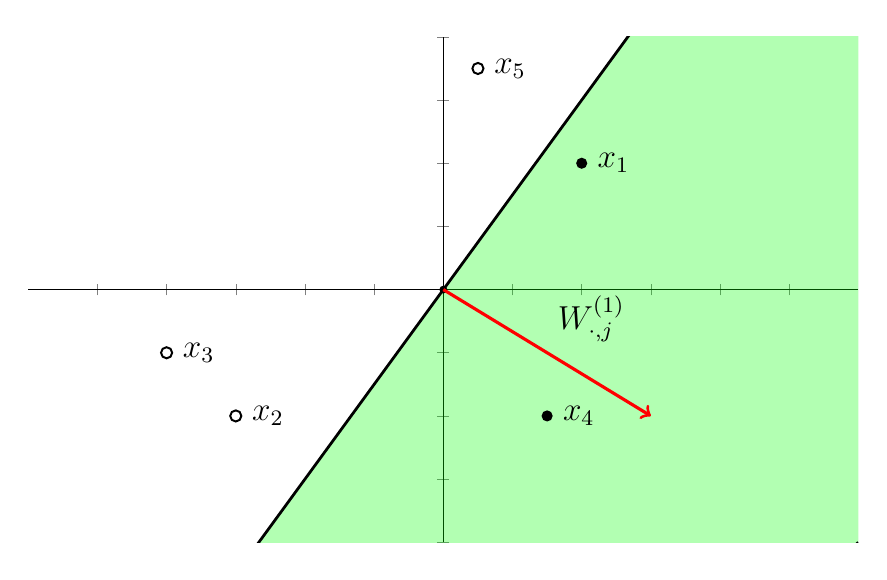
\begin{tikzpicture}[scale=1,
		declare function={
				cone_1(\x)= 3*\x/2;
				cone_2(\x)= -\x;
				cone_3(\x)= -4*\x;
				bounds(\x)= \x - 10;
			}
	]
	\begin{axis}[width=\linewidth, height=8cm,
			axis lines=center, yticklabels={,,}, xticklabels={,,},
			ymin=-4, ymax=4, ytick={-5,...,5}, ylabel=$$, x axis line style={-},
				xmin=-6, xmax=6, xtick={-5,...,5}, xlabel=$$, y axis line style={-},
		]
		\addplot[name path=cone_1, domain=-6:6, samples=100, line width=1pt]{cone_1(x)};
		\addplot[name path=bounds, domain=-6:6, samples=100, line width=1pt]{bounds(x)};

		% add color fill to both cones.

		\addplot fill between[
				of = cone_1 and bounds,
				%split, % calculate segment
				every even segment/.style = {fill=green, fill opacity=0.3},
			];

		%% point labels
		% origin point
		\node[circle, fill, inner sep=1pt] at (axis cs:0,0) {};

		% active examples 
		\node[label=right:$x_1$, circle, fill, inner sep=0.5mm] at (axis cs:2,2) {};
		\node[label=right:$x_4$, circle, fill, inner sep=0.5mm] at (axis cs:1.5,-2) {};

		% inactive examples 
		\node[label=right:$x_2$, circle, line width=0.25mm, draw=black, inner sep=0.5mm] at (axis cs:-3,-2) {};
		\node[label=right:$x_3$, circle, line width=0.25mm, draw=black, inner sep=0.5mm] at (axis cs:-4,-1) {};
		\node[label=right:$x_5$, circle, line width=0.25mm, draw=black, inner sep=0.5mm] at (axis cs:0.5,3.5) {};


		% lines
        \draw [->, draw=red, line width = 0.4mm] (axis cs:0,0) -- (axis cs:3,-2) node[midway,above right] {$W^{(1)}_{\cdot, j}$};
		%\draw [->, draw=red, line width = 0.4mm] (axis cs:2,-2) -- (axis cs:3,-1) node[midway,below right] {$S_{22} \cdot x_2$};
		%\draw [->, draw=red, line width = 0.4mm] (axis cs:0.5,-2) -- (axis cs:-2.5,-2.75) node[pos=0.9,below right] {$S_{33} \cdot x_3$};
	\end{axis}

\end{tikzpicture}%

        \else
            \Huge activation pattern figure
        \fi
    \end{figure}

    \phantom{
        \textbf{Activation Patterns} linearize ReLUs:
        \( D^{(1)}_j X W^{(1)}_{\cdot, j} = \rbr{X W^{(1)}_{\cdot, j}}_+ \)
    }

\end{frame}

\begin{frame}{Aside: ReLU Activation Patterns}

    Each ReLU neuron is active on a half-space: \( \rbr{X W^{(1)}_{\cdot, j}}_+ \)

    \begin{figure}[]
        \centering
        \ifdefined\showtikz
            %! TEX root = ../../main.tex

%% Illustration of cone decomposition. 

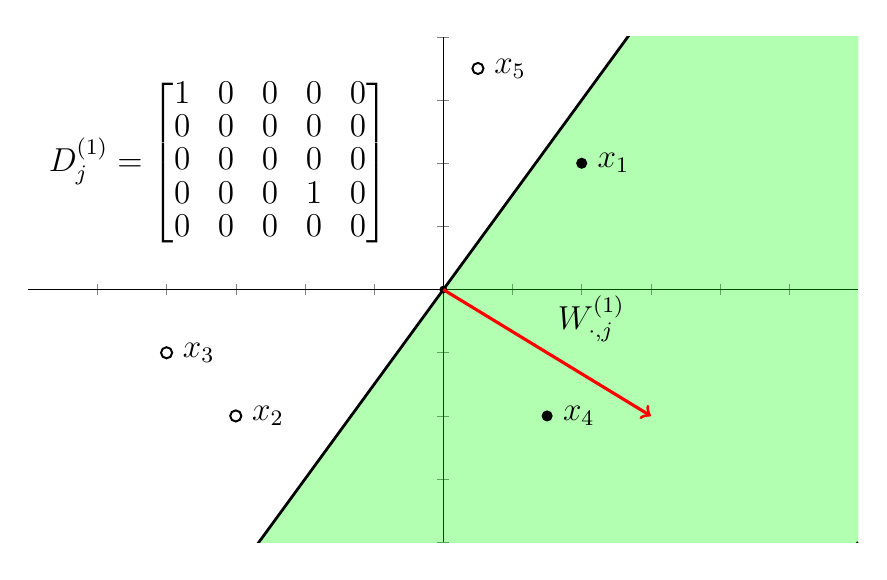
\begin{tikzpicture}[scale=1,
		declare function={
				cone_1(\x)= 3*\x/2;
				cone_2(\x)= -\x;
				cone_3(\x)= -4*\x;
				bounds(\x)= \x - 10;
			}
	]
	\begin{axis}[width=\linewidth, height=8cm,
			axis lines=center, yticklabels={,,}, xticklabels={,,},
			ymin=-4, ymax=4, ytick={-5,...,5}, ylabel=$$, x axis line style={-},
				xmin=-6, xmax=6, xtick={-5,...,5}, xlabel=$$, y axis line style={-},
		]
		\addplot[name path=cone_1, domain=-6:6, samples=100, line width=1pt]{cone_1(x)};
		\addplot[name path=bounds, domain=-6:6, samples=100, line width=1pt]{bounds(x)};

		% add color fill to both cones.

		\addplot fill between[
				of = cone_1 and bounds,
				%split, % calculate segment
				every even segment/.style = {fill=green, fill opacity=0.3},
			];

		%% point labels
		% origin point
		\node[circle, fill, inner sep=1pt] at (axis cs:0,0) {};

		% active examples 
		\node[label=right:$x_1$, circle, fill, inner sep=0.5mm] at (axis cs:2,2) {};
		\node[label=right:$x_4$, circle, fill, inner sep=0.5mm] at (axis cs:1.5,-2) {};

		% inactive examples 
		\node[label=right:$x_2$, circle, line width=0.25mm, draw=black, inner sep=0.5mm] at (axis cs:-3,-2) {};
		\node[label=right:$x_3$, circle, line width=0.25mm, draw=black, inner sep=0.5mm] at (axis cs:-4,-1) {};
		\node[label=right:$x_5$, circle, line width=0.25mm, draw=black, inner sep=0.5mm] at (axis cs:0.5,3.5) {};


		% activation pattern
		\node[] at (axis cs:-3.25,2) {
                $D^{(1)}_j = \begin{bmatrix}
					1 & 0 & 0 & 0 & 0 \\
					0 & 0 & 0 & 0 & 0 \\
					0 & 0 & 0 & 0 & 0 \\
					0 & 0 & 0 & 1 & 0 \\
					0 & 0 & 0 & 0 & 0 \\
				\end{bmatrix}
			$};

		% lines
        \draw [->, draw=red, line width = 0.4mm] (axis cs:0,0) -- (axis cs:3,-2) node[midway,above right] {$W^{(1)}_{\cdot, j}$};
		%\draw [->, draw=red, line width = 0.4mm] (axis cs:2,-2) -- (axis cs:3,-1) node[midway,below right] {$S_{22} \cdot x_2$};
		%\draw [->, draw=red, line width = 0.4mm] (axis cs:0.5,-2) -- (axis cs:-2.5,-2.75) node[pos=0.9,below right] {$S_{33} \cdot x_3$};
	\end{axis}

\end{tikzpicture}%

        \else
            \Huge activation pattern figure
        \fi
    \end{figure}

    \pause
    \textbf{Activation patterns} linearize ReLUs:
    \( \textcolor{brightpink}{\rbr{X W^{(1)}_{\cdot, j}}_+ = D^{(1)}_j X W^{(1)}_{\cdot, j}} \).

\end{frame}

\begin{frame}{Aside: ReLU Activation Patterns}

    Each ReLU neuron is active on a half-space: \( \rbr{X W^{(1)}_{\cdot, j}}_+ \)

    \begin{figure}[]
        \centering
        \ifdefined\showtikz
            %! TEX root = ../../main.tex

%% Illustration of cone decomposition. 

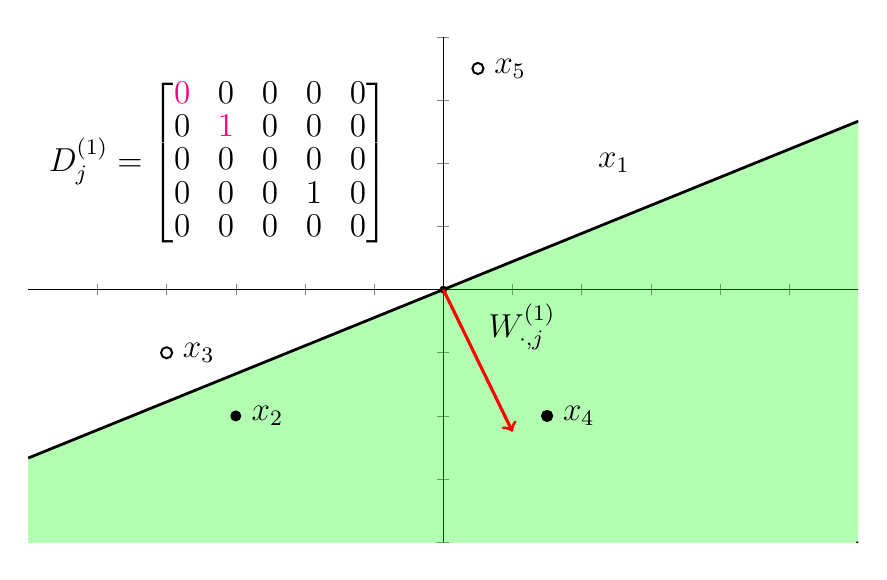
\begin{tikzpicture}[scale=1,
		declare function={
				cone_1(\x)= \x/2.25;
				cone_2(\x)= -\x;
				cone_3(\x)= -4*\x;
				bounds(\x)= \x - 10;
			}
	]
	\begin{axis}[width=\linewidth, height=8cm,
			axis lines=center, yticklabels={,,}, xticklabels={,,},
			ymin=-4, ymax=4, ytick={-5,...,5}, ylabel=$$, x axis line style={-},
				xmin=-6, xmax=6, xtick={-5,...,5}, xlabel=$$, y axis line style={-},
		]
		\addplot[name path=cone_1, domain=-6:6, samples=100, line width=1pt]{cone_1(x)};
		\addplot[name path=bounds, domain=-6:6, samples=100, line width=1pt]{bounds(x)};

		% add color fill to both cones.

		\addplot fill between[
				of = cone_1 and bounds,
				%split, % calculate segment
				every even segment/.style = {fill=green, fill opacity=0.3},
			];

		%% point labels
		% origin point
		\node[circle, fill, inner sep=1pt] at (axis cs:0,0) {};

		% active examples 
		\node[label=right:$x_1$, circle, line width=0.25mm, inner sep=0.5mm] at (axis cs:2,2) {};
		\node[label=right:$x_4$, circle, fill, draw=black, inner sep=0.5mm] at (axis cs:1.5,-2) {};

		% inactive examples 
		\node[label=right:$x_2$, circle, fill, inner sep=0.5mm] at (axis cs:-3,-2) {};
		\node[label=right:$x_3$, circle, line width=0.25mm, draw=black, inner sep=0.5mm] at (axis cs:-4,-1) {};
		\node[label=right:$x_5$, circle, line width=0.25mm, draw=black, inner sep=0.5mm] at (axis cs:0.5,3.5) {};


		% activation pattern
		\node[] at (axis cs:-3.25,2) {
                $D^{(1)}_j = \begin{bmatrix}
                \textcolor{brightpink}{0} & 0        & 0 & 0 & 0 \\
                0       & \textcolor{brightpink}{1} & 0 & 0 & 0 \\
					0       & 0        & 0 & 0 & 0 \\
					0       & 0        & 0 & 1 & 0 \\
					0       & 0        & 0 & 0 & 0 \\
				\end{bmatrix}
			$};

		% lines
        \draw [->, draw=red, line width = 0.4mm] (axis cs:0,0) -- (axis cs:1,-2.25) node[midway,above right] {$W^{(1)}_{\cdot, j}$};

	\end{axis}

\end{tikzpicture}%

        \else
            \Huge activation pattern figure
        \fi
    \end{figure}

    \textbf{Activation patterns} linearize ReLUs:
    \( \textcolor{brightpink}{\rbr{X W^{(1)}_{\cdot, j}}_+
        = D^{(1)}_j X W^{(1)}_{\cdot, j}} \).

\end{frame}

\begin{frame}{Convex Reformulations: Convex Problem}

    {\large \good{Convex Reformulation} (C-ReLU)} \citep{pilanci2020convex}
    \[
        \begin{aligned}
            \min_{v, w} & \half \norm{\sum_{j=1}^{p_1} \textcolor{brightpink}{D^{(1)}_j X (v_j - w_j)} - y}_2^2 +
            \lambda \sum_{j=1}^{p_1} \norm{v_j}_2 + \norm{w_j}_2                                                  \\
                        & \hspace{0.2em} \text{s.t. }
            \textcolor{brightpink}{v_j, w_j \in \calK^{(1)}_j} :=
            \big\{w : \underbrace{(2D^{(1)}_j - I) X w \geq 0}_{\iff \rbr{X w}_+ = D^{(1)}_j X w}\big\},
        \end{aligned}
    \]
    where \( p_1 \) is the number of unique activation patterns.
    \pause

    \begin{figure}[]
        \centering
        \ifdefined\showtikz
            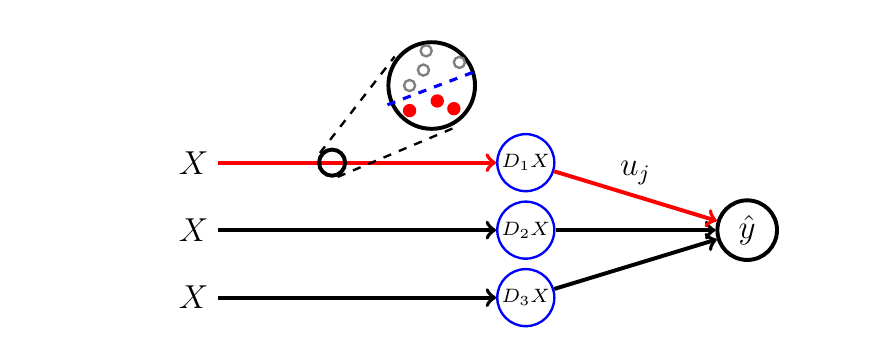
\begin{tikzpicture}[scale=1,
	]
	\begin{axis}[width=\linewidth, height=5.5cm,
			axis lines=none,  % don't print axis lines
			yticklabels={,,}, xticklabels={,,},
			ymin=0, ymax=8, y axis line style={-},
			xmin=0, xmax=15, x axis line style={-},
		]
		\node [] (input1) at (axis cs:3,1) {$X$};
		\node [] (input2) at (axis cs:3,2.75) {$X$};
		\node [] (input3) at (axis cs:3,4.5) {$X$};

        \node [Splits] (hidden1) at (axis cs:9,1) {\scriptsize $D_3 X$};
		\node [Splits] (hidden2) at (axis cs:9,2.75) {\scriptsize $D_2 X$};
		\node [Splits] (hidden3) at (axis cs:9,4.5) {\scriptsize $D_1 X$};

		\draw [->, style=arrow, draw=black] (input1) -- (hidden1);

		\draw [->, style=arrow, draw=black] (input2) -- (hidden2);

		\draw [->, style=arrow, draw=red] (input3) -- (hidden3);

		\node [Output] (output) at (axis cs:13,2.75) {$\hat y$};

		\draw [->, style=arrow, draw=black] (hidden1) -- (output);
		\draw [->, style=arrow, draw=black] (hidden2) -- (output);
		\draw [->, style=arrow, draw=red] (hidden3) -- (output) node[pos=0.5,above] {$u_j$};

		\draw [draw=black, line width=0.3mm, dashed] (axis cs:5.6, 4.13) -- (axis cs:7.7,5.4);
		\draw [draw=black, line width=0.3mm, dashed] (axis cs:5.28, 4.75) -- (axis cs:6.63,7.25);

		\node [draw=black, minimum size=0.3cm, shape=circle, solid, line width=0.5mm] (examine) at (axis cs:5.5,4.5) {};
		\node [draw=black, minimum size=1.1cm, shape=circle, solid, line width=0.5mm] (closeup) at (axis cs:7.3,6.5) {};

		\node [fill=white, draw=gray, line width=0.3mm, inner sep=0.05cm, shape=circle] at (axis cs:7.8,7.1) {};
		\node [fill=white, draw=gray, line width=0.3mm, inner sep=0.05cm, shape=circle] at (axis cs:7.15,6.9) {};
		\node [fill=white, draw=gray, line width=0.3mm, inner sep=0.05cm, shape=circle] at (axis cs:7.2,7.4) {};
		\node [fill=white, draw=gray, line width=0.3mm, inner sep=0.05cm, shape=circle] at (axis cs:6.9,6.5) {};

		\draw [draw=Blue, dashed, line width=0.4mm] (axis cs:6.5,6.) -- (axis cs:8.15,6.9);

		\node [fill=Red, inner sep=0.06cm, shape=circle] at (axis cs:6.9,5.85) {};
		\node [fill=Red, inner sep=0.06cm, shape=circle] at (axis cs:7.4,6.1) {};
		\node [fill=Red, inner sep=0.06cm, shape=circle] at (axis cs:7.7,5.9) {};

	\end{axis}

\end{tikzpicture}%

%\begin{tikzpicture}[scale=1,
%    ]
%    \begin{axis}[width=1.1\linewidth, height=5cm,
%            axis lines=none,  % don't print axis lines
%            yticklabels={,,}, xticklabels={,,},
%            ymin=-0.2, ymax=10.2, x axis line style={-},
%            xmin=-0.2, xmax=20.2, y axis line style={-},
%        ]

%        \filldraw[color=blue!60, fill=blue!5, line width=0.4mm](axis cs:0,5.8) rectangle (axis cs:20, 10);
%        \filldraw[color=red!60, fill=red!5, line width=0.4mm](axis cs:0,0) rectangle (axis cs:20, 4.2);

%        % non-convex models
%        \filldraw[line width=0.4mm, fill=white](axis cs:1,1) rectangle (axis cs:8, 3.2) node[pos=.5] {NC-GReLU};
%        \filldraw[line width=0.4mm, fill=white](axis cs:12,1) rectangle (axis cs:19, 3.2) node[pos=.5] {NC-ReLU};

%        % convex models
%        \filldraw[line width=0.4mm, fill=white](axis cs:1,6.8) rectangle (axis cs:8, 9) node[pos=.5] {C-GReLU};
%        \filldraw[line width=0.4mm, fill=white](axis cs:12,6.8) rectangle (axis cs:19, 9) node[pos=.5] {C-ReLU};

%        \draw [<->, solid, draw=black, line width = 0.6mm] (axis cs:4.5,3.2) -- (axis cs:4.5,6.8) node[right, pos=0.5] {\small Sol. Map};

%        \draw [<->, solid, draw=black, line width = 0.6mm] (axis cs:15.5,3.2) -- (axis cs:15.5,6.8)  node[right, pos=0.5] {\small Sol. Map};

%        \draw [<-, solid, draw=black, line width = 0.6mm] (axis cs:6,9) -- [bend left=15] (axis cs:14, 9);

%        \draw [->, solid, draw=orange, line width = 0.6mm] (axis cs:8,7.9) -- (axis cs:12,7.9);
%        \node[align=center] at (axis cs:10.1, 7.8) {\small Cone\\ \small Decomp.};
%    \end{axis}

%\end{tikzpicture}%


        \else
            \Huge convex reformulation figure
        \fi
    \end{figure}
\end{frame}

\begin{frame}{Convex Reformulations: Hardness}

    \textbf{Key Result}: if network width \( m \) satisfies \( m \geq m^* \)
    for some \( m^* \leq n \), then C-ReLU and NC-ReLU are \good{equivalent}
    \citep{pilanci2020convex}.

    \pause
    \horizontalrule

    How \textbf{hard} is the convex program?
    \pause

    \[
        p_1 = \abs{\cbr{D_j = \text{diag}[\mathbbm{1}(X g_j \geq 0)] : g_j \in \R^d }}
    \]

    \vspace{2em}
    \pause

    The \textbf{convex program} is:
    \vspace{0.5em}
    \begin{itemize}
        \item \bad{Exponential in general}: \( p_1 \in O(r \cdot (\frac{n}{r})^r) \),
              where \( r = \text{rank}(X) \).

              \pause
              \vspace{1em}

        \item \good{Highly structured} --- it's a linear model!
    \end{itemize}

    \vspace{1em}
    \pause

    \textbf{Takeaway}: We exchange one kind of hardness for another.

\end{frame}

\setbeamercolor{background canvas}{bg=LightCyan}
\begin{frame}{}
    \begin{center}
        \huge
        3. Deep Convex Reformulations
    \end{center}
\end{frame}
\setbeamercolor{background canvas}{bg=white}

\begin{frame}{Deep Networks: Big Idea}

    \textbf{Big Idea}: Extend convex reformulations to \good{deep ReLU
        networks}.

    \pause
    \vspace{1ex}
    \begin{columns}
        \column{0.5\textwidth}
        \begin{itemize}
            \item<2-> Previous work is limited to \bad{deep parallel
                      networks} \citep{ergen2021global, wang2023parallel}.
                  \vspace{1ex}

            \item<3-> We abandon strong duality and argue by \good{reductions}.
        \end{itemize}
        \column{0.5\textwidth}
        \begin{center}
            \def\layersep{1.25cm}
\begin{tikzpicture}[shorten >=1pt,->,draw=black!50, node distance=\layersep]
    \tikzstyle{every pin edge}=[<-,shorten <=1pt]
    \tikzstyle{neuron}=[circle,fill=black!25,minimum size=7pt,inner sep=0pt]
    \tikzstyle{rect}= [rectangle, draw=black!50, thick, minimum width=0.5cm, minimum height=1.7cm]
    \tikzstyle{input neuron}=[neuron, fill=green!50];
    \tikzstyle{output neuron}=[neuron, fill=red!50];
    \tikzstyle{hidden neuron}=[neuron, fill=blue!50];
    \tikzstyle{hidden neuron2}=[neuron, fill=orange!50];
    \tikzstyle{hidden neuron3}=[neuron, fill=purple!50];
    \tikzstyle{annot} = [text width=4em, text centered]

    % Draw the input layer nodes
    \foreach \name / \y in {1,...,3}
    % This is the same as writing \foreach \name / \y in {1/1,2/2,3/3,4/4}
    \node[input neuron] (I-\name) at (0,-\y/2-0.25) {};

    % Draw the hidden layer nodes
    \foreach \name / \y in {1,...,8}
    \path[yshift=2cm]
    node[hidden neuron] (H-1-\name) at (\layersep,-\y/2-1) {};
    \node[rect, minimum height=1.9cm] (L1-1) at (\layersep,-0.25) {};
    \node[rect, minimum height=1.9cm] (L1-2) at (\layersep,-2.25) {};
    \foreach \name / \y in {1,...,6}
    \path[yshift=1.5cm]
    node[hidden neuron2] (H-2-\name) at (2*\layersep,-\y/2-1) {};
    \node[rect, minimum height=1.4cm] (L2-1) at (2*\layersep,-0.5) {};
    \node[rect, minimum height=1.4cm] (L2-2) at (2*\layersep,-2) {};
    \foreach \name / \y in {1,...,2}
    \path[yshift=0.5cm]
    node[hidden neuron3] (H-3-\name) at (3*\layersep,-\y/2-1) {};
    \node[rect, minimum height=0.4cm] (L3-1) at (3*\layersep,-1) {};
    \node[rect, minimum height=0.4cm] (L3-1) at (3*\layersep,-1.5) {};
    % Draw the output layer node
    \foreach \name / \y in {1,...,2}
    \path[yshift=0.5cm]
    node[output neuron] (O-\name) at (4*\layersep,-\y/2-1) {};
    \node[rect, minimum height=0.9cm] (L4) at (4*\layersep,-1.25) {};

    % Connect every node in the input layer with every node in the
    % hidden layer.
    \foreach \source in {1,...,3}
    \foreach \dest in {1,...,8}
    \path (I-\source) edge (H-1-\dest);

    \foreach \source in {1,...,4}
    \foreach \dest in {1,...,3}
    \path (H-1-\source) edge (H-2-\dest);
    \foreach \source in {5,...,8}
    \foreach \dest in {4,...,6}
    \path (H-1-\source) edge (H-2-\dest);

    % Connect every node in the hidden layer with the output layer
    \foreach \source in {1,...,2}
    \foreach \dest in {1,...,2}
    \path (H-3-\source) edge (O-\dest);

    \foreach \source in {1,...,3}
    \foreach \dest in {1,...,1}
    \path (H-2-\source) edge (H-3-\dest);
    \foreach \source in {4,...,6}
    \foreach \dest in {2,...,2}
    \path (H-2-\source) edge (H-3-\dest);

    % Annotate the layers
    %\node[annot,above of=H-1-1, node distance=0.5cm] (hl) {Layer 1};
    %\node[annot,left of=hl] {Input};
    %\node[annot,above of=H-2-1, node distance=1cm](hl2) {Layer 2};
    %\node[annot,right of=hl2](hl3) {Layer 3};
    %\node[annot,right of=hl3](hl4) {Layer 4};
\end{tikzpicture}

            %Parallel Neural Network
        \end{center}
    \end{columns}

    \vspace{-1ex}
    \pause
    \pause
    \textbf{Hierarchy of Difficulty}
    \pause
    \begin{columns}[c]
        \begin{column}{0.33\textwidth}
            \begin{center}
                \underline{Linear Models}
                \vspace{0.4ex}

                \good{Linear} combination of inputs.
            \end{center}
        \end{column}
        \pause
        \begin{column}{0.33\textwidth}
            \begin{center}
                \underline{Two-Layer Networks}
                \vspace{0.4ex}

                \good{Linear} combination of \bad{non-linear}.
            \end{center}
        \end{column}
        \pause
        \begin{column}{0.34\textwidth}
            \begin{center}
                \underline{\( L \)-Layer Networks}
                \vspace{0.4ex}

                \bad{Non-linear} combin.\ of \bad{non-linear}.
            \end{center}
        \end{column}
    \end{columns}

    \source{Figure taken from \citet{kim2025exploring}.}

    %\begin{itemize}
    %    \item<4-> Three layer networks have \bad{non-linear}
    %          combinations of \bad{non-linear} functions, which are challenging
    %          to analyze.
    %          \pause
    %          \vspace{0.5ex}

    %    \item But, once we understand \good{three layer} networks, we understand
    %          \good{\( k \)-layer} networks for any \( k \geq 3 \).
    %          \pause
    %          \vspace{0.5ex}

    %    \item  We prove that ReLU MLPs of arbitrary depth are \good{convex
    %              functions} with non-convex \bad{tensor decomposition} constraints.

    %\end{itemize}

\end{frame}

\begin{frame}{Deep Networks: Layer Elimination}

    Let \( W^{(l)} \in \R^{d_{l-1} \times d_l} \) and
    consider the \( k \)-layer ReLU network
    \[
        f_\theta(X) =
        \rbr{\rbr{\textcolor{brightpink}{\rbr{X W^{(1)}}_+ W^{(2)}}}_+ W^{(3)} \cdots }_+ W^{(k)}.
    \]

    \pause
    \horizontalrule

    \textbf{Question}: how do we construct a \good{convex reformulation}?

    \pause
    \vspace{1ex}

    \begin{enumerate}
        \item The first \good{two-layer block} has a convex reformulation,
              \[
                  f_\theta(X) = \rbr{\rbr{
                          \textcolor{brightpink}{\sum_{i=1}^p D^{(1)}_i X T_i^{(2)}}}_+
                      \otimes W_i^{(3)} \cdots }_+ W^{(k)}.
              \]
              \pause
              \vspace{0.5ex}

        \item This creates another \good{two-layer block}, which has a convex
              reformulation in terms of
              \( X^{(2)} = [D_1^{(1)} X \ldots D_{p_1}^{(1)} X] \).
    \end{enumerate}

\end{frame}

\begin{frame}{Deep Networks: Tensor Programs}

    Let \( T^{(l)} \in \R^{d_0 \times p_1 \times \cdots \times p_{l-1} \times d_{l}}
    \) be a tensor in the low-rank set,
    \[
        \calG^{(l)} = \cbr{ T^{(l)} :
            \exists \, T^{(l-1)} \in \calG^{(l-1)} \text{ s.t. }
            T^{(l)}_j = \!\!\!\!\!\!\!\! \sum_{T^{(l-1)}_i \in \calK^{(l-1)}_j }
            T_i^{(l-1)} \otimes W^{(l)}_i.
        }
    \]
    \vspace{-1ex}
    \pause

    \begin{beamercolorbox}[wd=\textwidth,sep=1em]{result}
        \textbf{Proposition}:
        Training an \( L \)-layer ReLU model,
        \begin{equation*}
            \min_{\theta} \calL\rbr{f_{\theta}(X), y},
        \end{equation*}
        is equivalent to solving the order \( L+1 \) tensor program
        \begin{equation*}
            \min_{T^{(L)}} \, \calL\rbr{X^{(L)} \odot T^{(L)}, y}
            \quad \text{s.t.} \quad \textcolor{brightpink}{T^{(L)} \in \calG^{(L)}}.
        \end{equation*}
        \vspace{-3ex}
    \end{beamercolorbox}
    \pause

    \begin{itemize}
        \item Prediction is a \good{linear operation} on tensors:
              \[
                  X^{(L)} \odot T^{(L)} = \sum_{j_1, \ldots, j_{L-1}}
                  D^{(1)}_{j_1} \cdots D^{(L-1)}_{j_{L-1}} X T^{(L)}_{j_1, \ldots, j_L-1}
              \]
    \end{itemize}

\end{frame}

\begin{frame}{Deep Networks: Fully Convex Version}
    \[
        \calG^{(l)} = \cbr{ T^{(l)} :
            \exists \, T^{(l-1)} \in \calG^{(l-1)} \text{ s.t. }
            T^{(l)}_j = \!\!\!\!\!\!\!\! \textcolor{brightpink}{
                \sum_{T^{(l-1)}_i \in \calK^{(l-1)}_j }
                T_i^{(l-1)} \otimes W^{(l)}_i}.
        }
    \]
    \pause
    \begin{itemize}
        \item If \( d_l \geq 2 p_l d_{l+1} \) for every \( l \), then \( \calG^{(L)} \)
              becomes \good{fully convex}.
    \end{itemize}

    \pause
    \horizontalrule

    \begin{beamercolorbox}[wd=\textwidth,sep=1em]{result}
        \textbf{Theorem}:
        If \( m_{l} \geq m^*_l  \) for some threshold
        \textcolor{brightpink}{\(m^*_l \leq 3n \)}, then
        \begin{equation*}
            \min_{\theta} \calL\rbr{f_{\theta}(X), y},
        \end{equation*}
        is equivalent to solving the unconstrained tensor program
        \begin{equation*}
            \min_{T^{(L)}} \, \calL\rbr{X^{(L)} \odot T^{(L)}, y}.
        \end{equation*}
    \end{beamercolorbox}

\end{frame}

\begin{frame}{Deep Networks: Tensor Parameterization}

    \textbf{Q}: What does the tensor \( T^{(L)} \) represent?
    \pause
    \vspace{1ex}

    \textbf{A}: Each entry \( T^{(L)}_{i_0, i_1, \ldots, i_{L}} \) is a
    path in the network DAG given by
    \[
        T^{(L)}_{i_0, i_1, \ldots, i_{k}}
        = W^{(1)}_{i_0, i_1} \cdot W^{(2)}_{i_1, i_2} \cdots W^{(L)}_{i_{L-1}, i_L}.
    \]

    \vspace{-3ex}
    \pause
    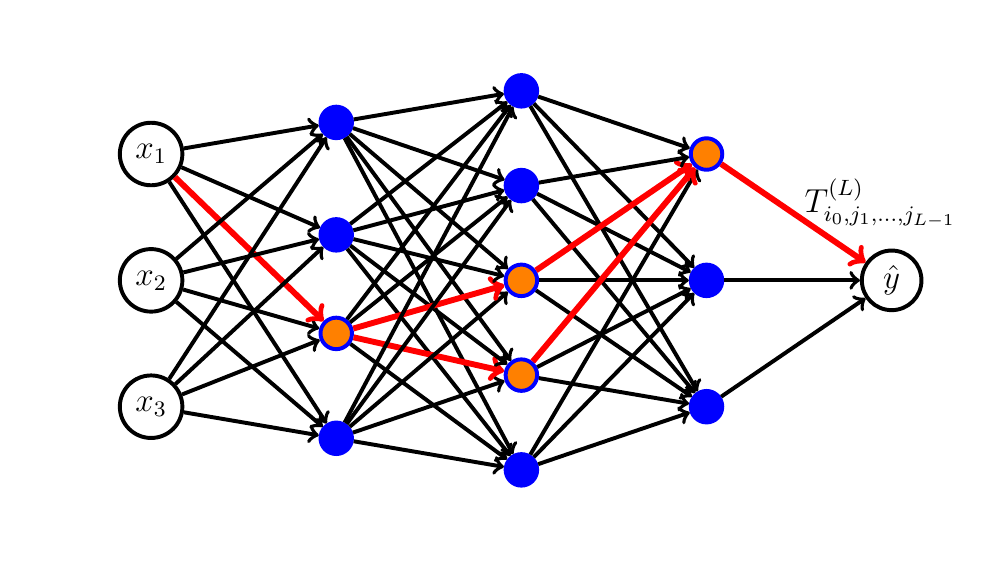
\begin{tikzpicture}[scale=1,
	]
	\begin{axis}[width=1.1\textwidth, height=8cm,
			axis lines=none,  % don't print axis lines
			yticklabels={,,}, xticklabels={,,},
			ymin=0, ymax=8, y axis line style={-},
			xmin=0, xmax=15, x axis line style={-},
		]
		%\node [] (input) at (axis cs:1,4) {$X$};
		\node [Input] (input1) at (axis cs:2,2) {$x_3$};
		\node [Input] (input2) at (axis cs:2,4) {$x_2$};
		\node [Input] (input3) at (axis cs:2,6) {$x_1$};

		%\draw [decorate, line width = 0.6mm,
		%    decoration = {calligraphic brace}] (axis cs:2,1.5) --  (axis cs:2,6.5);

		\node [Hidden] (hidden11) at (axis cs:5,1.5) {};
		\node [Hidden, fill=orange] (hidden12) at (axis cs:5,3.16) {};
		\node [Hidden] (hidden13) at (axis cs:5,4.72) {};
		\node [Hidden] (hidden14) at (axis cs:5,6.5) {};

		\node [Hidden] (hidden21) at (axis cs:8,1) {};
		\node [Hidden, fill=orange] (hidden22) at (axis cs:8,2.5) {};
		\node [Hidden, fill=orange] (hidden23) at (axis cs:8,4) {};
		\node [Hidden] (hidden24) at (axis cs:8,5.5) {};
		\node [Hidden] (hidden25) at (axis cs:8,7) {};

		\node [Hidden] (hidden31) at (axis cs:11,2) {};
		\node [Hidden] (hidden32) at (axis cs:11,4) {};
		\node [Hidden, fill=orange] (hidden33) at (axis cs:11,6) {};

		\node [Output] (output) at (axis cs:14,4) {$\hat y$};

		% Layer 1

		\draw [->, style=arrow, draw=black] (input1) -- (hidden11);
		\draw [->, style=arrow, draw=black] (input2) -- (hidden11);
		\draw [->, style=arrow, draw=black] (input3) -- (hidden11);

		\draw [->, style=arrow, draw=black] (input1) -- (hidden12);
		\draw [->, style=arrow, draw=black] (input2) -- (hidden12);
		\draw [->, style=arrow, draw=red, line width = 0.75mm] (input3) -- (hidden12);

		\draw [->, style=arrow, draw=black] (input1) -- (hidden13);
		\draw [->, style=arrow, draw=black] (input2) -- (hidden13);
		\draw [->, style=arrow, draw=black] (input3) -- (hidden13);

		\draw [->, style=arrow, draw=black] (input1) -- (hidden14);
		\draw [->, style=arrow, draw=black] (input2) -- (hidden14);
		\draw [->, style=arrow, draw=black] (input3) -- (hidden14);

		% Layer 2

		\draw [->, style=arrow, draw=black] (hidden11) -- (hidden21);
		\draw [->, style=arrow, draw=black] (hidden12) -- (hidden21);
		\draw [->, style=arrow, draw=black] (hidden13) -- (hidden21);
		\draw [->, style=arrow, draw=black] (hidden14) -- (hidden21);

		\draw [->, style=arrow, draw=black] (hidden11) -- (hidden22);
		\draw [->, style=arrow, draw=red, line width = 0.75mm] (hidden12) -- (hidden22);
		\draw [->, style=arrow, draw=black] (hidden13) -- (hidden22);
		\draw [->, style=arrow, draw=black] (hidden14) -- (hidden22);

		\draw [->, style=arrow, draw=black] (hidden11) -- (hidden23);
		\draw [->, style=arrow, draw=red, line width = 0.75mm] (hidden12) -- (hidden23);
		\draw [->, style=arrow, draw=black] (hidden13) -- (hidden23);
		\draw [->, style=arrow, draw=black] (hidden14) -- (hidden23);

		\draw [->, style=arrow, draw=black] (hidden11) -- (hidden24);
		\draw [->, style=arrow, draw=black] (hidden12) -- (hidden24);
		\draw [->, style=arrow, draw=black] (hidden13) -- (hidden24);
		\draw [->, style=arrow, draw=black] (hidden14) -- (hidden24);

		\draw [->, style=arrow, draw=black] (hidden11) -- (hidden25);
		\draw [->, style=arrow, draw=black] (hidden12) -- (hidden25);
		\draw [->, style=arrow, draw=black] (hidden13) -- (hidden25);
		\draw [->, style=arrow, draw=black] (hidden14) -- (hidden25);

		% Layer 3

		\draw [->, style=arrow, draw=black] (hidden21) -- (hidden31);
		\draw [->, style=arrow, draw=black] (hidden22) -- (hidden31);
		\draw [->, style=arrow, draw=black] (hidden23) -- (hidden31);
		\draw [->, style=arrow, draw=black] (hidden24) -- (hidden31);
		\draw [->, style=arrow, draw=black] (hidden25) -- (hidden31);

		\draw [->, style=arrow, draw=black] (hidden21) -- (hidden32);
		\draw [->, style=arrow, draw=black] (hidden22) -- (hidden32);
		\draw [->, style=arrow, draw=black] (hidden23) -- (hidden32);
		\draw [->, style=arrow, draw=black] (hidden24) -- (hidden32);
		\draw [->, style=arrow, draw=black] (hidden25) -- (hidden32);

		\draw [->, style=arrow, draw=black] (hidden21) -- (hidden33);
		\draw [->, style=arrow, draw=red, line width = 0.75mm] (hidden22) -- (hidden33);
		\draw [->, style=arrow, draw=red, line width = 0.75mm] (hidden23) -- (hidden33);
		\draw [->, style=arrow, draw=black] (hidden24) -- (hidden33);
		\draw [->, style=arrow, draw=black] (hidden25) -- (hidden33);

		\draw [->, style=arrow, draw=black] (hidden31) -- (output);
		\draw [->, style=arrow, draw=black] (hidden32) -- (output);
		\draw [->, style=arrow, draw=red, line width = 0.75mm] (hidden33) -- (output) node[pos=0.4,right] {\hspace{0.2ex} $T^{(L)}_{i_0, j_1, \ldots, j_{L-1}, i_L}$};

		%\draw [->, style=arrow, draw=black] (hidden4) -- (output) node[pos=0.5,above] {$w_{2j}$};
	\end{axis}

\end{tikzpicture}%


\end{frame}

\setbeamercolor{background canvas}{bg=LightCyan}
\begin{frame}{}
    \begin{center}
        \huge 4. Polynomial Time Fitting
    \end{center}
\end{frame}
\setbeamercolor{background canvas}{bg=white}

\begin{frame}{Poly-Time Fitting: Complexity}
    The tensor \( T^{(L)} \) is a
    \( \good{d} \times \bad{p_1 \times \cdots \times p_{L-1}} \times \good{c} \)
    dimensional.

    \vspace{1ex}
    \pause

    \begin{itemize}
        \item \( \bad{p_l} \) is the number of activation patterns \(
              D^{(l)}_{j} \) in the \( l^{\text{th}} \) layer.

              \vspace{1ex}
              \pause

              \begin{itemize}
                  \item \( \bad{p_l = \abs{\calD^{(l)}}} \), where
                        \( \calD^{(l)} = \cbr{ \text{diag}
                            \rbr{\mathds{1}\rbr{f_{\theta_{l}}(X) \geq 0}}
                            : \theta \in \Delta_{l}} \)
              \end{itemize}

              \vspace{2ex}
              \pause

        \item We know \( p_1 \leq 2 r (e \frac{n-1}{r})^r \), where
              \( r := \text{rank}(X) \) \citep{pilanci2020convex}.

              \vspace{1ex}
              \pause

              \begin{itemize}
                  \item This is \good{polynomial} when \( d \) is fixed!
              \end{itemize}

              \vspace{2ex}
              \pause

        \item What about \( p_l \) for \( l \geq 2 \)?

              \vspace{1ex}
              \pause

              \begin{itemize}
                  \item If \( f_{\theta_l} \) can \underline{shatter} \( X \),
                        then we must have \( p_l = 2^{n} \)!
              \end{itemize}
    \end{itemize}

    \vspace{1ex}
    \pause
    \horizontalrule

    \begin{center}
        \large
        \textbf{Easier Problem}:
        when can \( f_{\theta_l} \) exactly interpolate \( \rbr{X, y}? \)
    \end{center}

\end{frame}

\begin{frame}{Poly-Time Fitting: Interpolation without Biases}

    \begin{columns}
        \begin{column}{0.5\textwidth}
            \begin{beamercolorbox}[wd=\textwidth,sep=1em]{result}
                \textbf{Proposition}:
                If \( x_i \neq \alpha x_j \) for any \( i \neq j \), then there
                exists a two-layer neural network with at most \( 3n \) neurons
                such that \( f_\theta(X) = y \).
            \end{beamercolorbox}
        \end{column}
        \begin{column}{0.5\textwidth}
            \begin{figure}
                \centering
                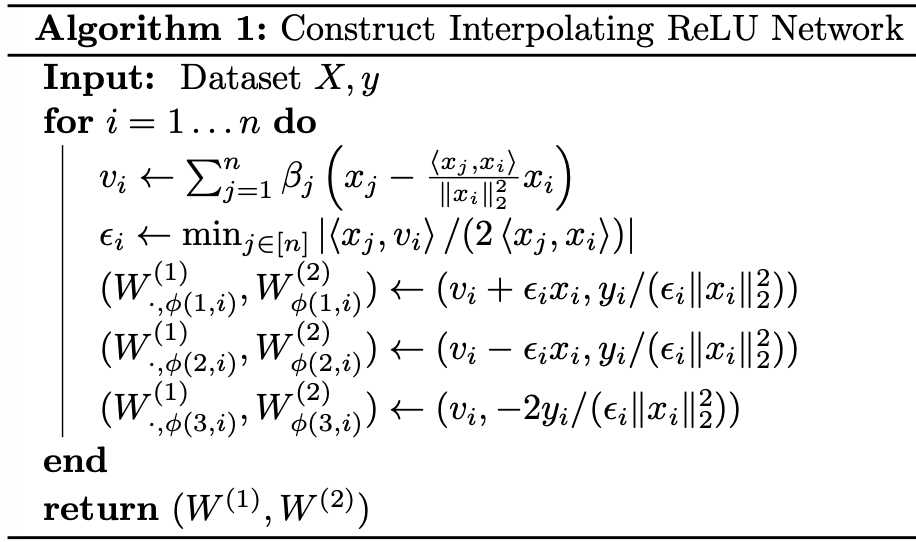
\includegraphics[width=\textwidth]{assets/interpolation_alg.png}
            \end{figure}
        \end{column}
    \end{columns}

    \pause
    \vspace{1ex}

    \begin{itemize}
        \item This is a \underline{bias-free} version of the interpolation result from
              \citet{zhang2017understanding}.

              \pause
              \vspace{1ex}

        \item \textbf{Key Idea}: if \( x_i \) is not collinear with any \( x_j \),
              then there exists \( D^{(1)}_l \) and \( D^{(1)}_k \) with
              \( D^{(1)}_l - D^{(1)}_k = \text{diag}(e_i) \).

              \pause
              \vspace{1ex}

        \item \textbf{Corollary}: wide two-layer networks can \good{shatter}
              data up to group of \bad{collinear examples}.
    \end{itemize}

    \source{Algorithm conceived jointly with Christoph Hertrich.}

\end{frame}

\begin{frame}{Poly-Time Fitting: Size of Reformulation}
    \begin{beamercolorbox}[wd=\textwidth,sep=1em]{result}
        \textbf{Proposition}: If \( r := \text{rank}\,(X) \) and
        \( n_s = \abs{\cbr{x_i / \norm{x_i} : i \in [n]}} \), then
        the number of activation patterns satisfies
        \begin{equation*}\label{eq:activation-pattern-bound}
            p_l \quad
            \begin{cases}
                \leq 2 r \rbr{e \frac{n - 1}{r}}^{r} & \mbox{if \( l = 1 \)}  \\
                = 2^{n_{s}}                          & \mbox{if \( l > 1 \)}.
            \end{cases}
        \end{equation*}
    \end{beamercolorbox}

    \pause
    \vspace{2ex}

    \textbf{Positive}: the expressivity of the model on \( X \) stagnates
    after \( l = 3 \).

    \pause
    \vspace{2ex}

    \textbf{Negative}: the convex reformulation is \bad{exponential
        size} unless only \( \log(n) \) examples have unique (signed) directions.

    \pause
    \vspace{2ex}

    \textbf{What Next?} Is polynomial time fitting still possible?

    \pause
    \vspace{1ex}

    \begin{itemize}
        \item[$\longrightarrow$] \good{Yes!} But we need restrict the
              activations to a basis of \( D^{(l)} \).
    \end{itemize}

\end{frame}

\begin{frame}{Poly-Time Fitting: Representative Activations}

    \textbf{Approach}: use differences \( D^{(l)}_i - D^{(l)}_j \)
    to build a basis.

    \vspace{1ex}
    \pause

    \begin{itemize}
        \item Let \( n_u \) be the number of unsigned directions in \( X \).
    \end{itemize}

    \vspace{1ex}
    \pause

    \begin{beamercolorbox}[wd=\textwidth,sep=1em]{result}
        \textbf{Lemma}: There exists \( \tilde{D} \) with at most
        \( \min\cbr{n, 2 n_u} \) activation patterns such that
        \( \tilde{D} \) is a basis for \( \calD^{(l)} \).
    \end{beamercolorbox}

    \vspace{1ex}
    \pause

    \begin{beamercolorbox}[wd=\textwidth,sep=1em]{result}
        \textbf{Theorem}: A global solution to the \( L \)-layer
        ReLU network training problem
        \[
            \min_{\theta} \calL(f_\theta(X), y),
        \]
        can be computed in \( O(n^2 d + n^3 + nc) \) time.
    \end{beamercolorbox}
    \pause

    \begin{itemize}
        \item Does not contradict \bad{NP-Hardness} because
              layers are \good{wide}: \( m_l \geq \min\cbr{n, 2n_u} \).
    \end{itemize}

\end{frame}

\begin{frame}{Poly-Time Fitting: Exact Training}

    \begin{figure}
        \centering
        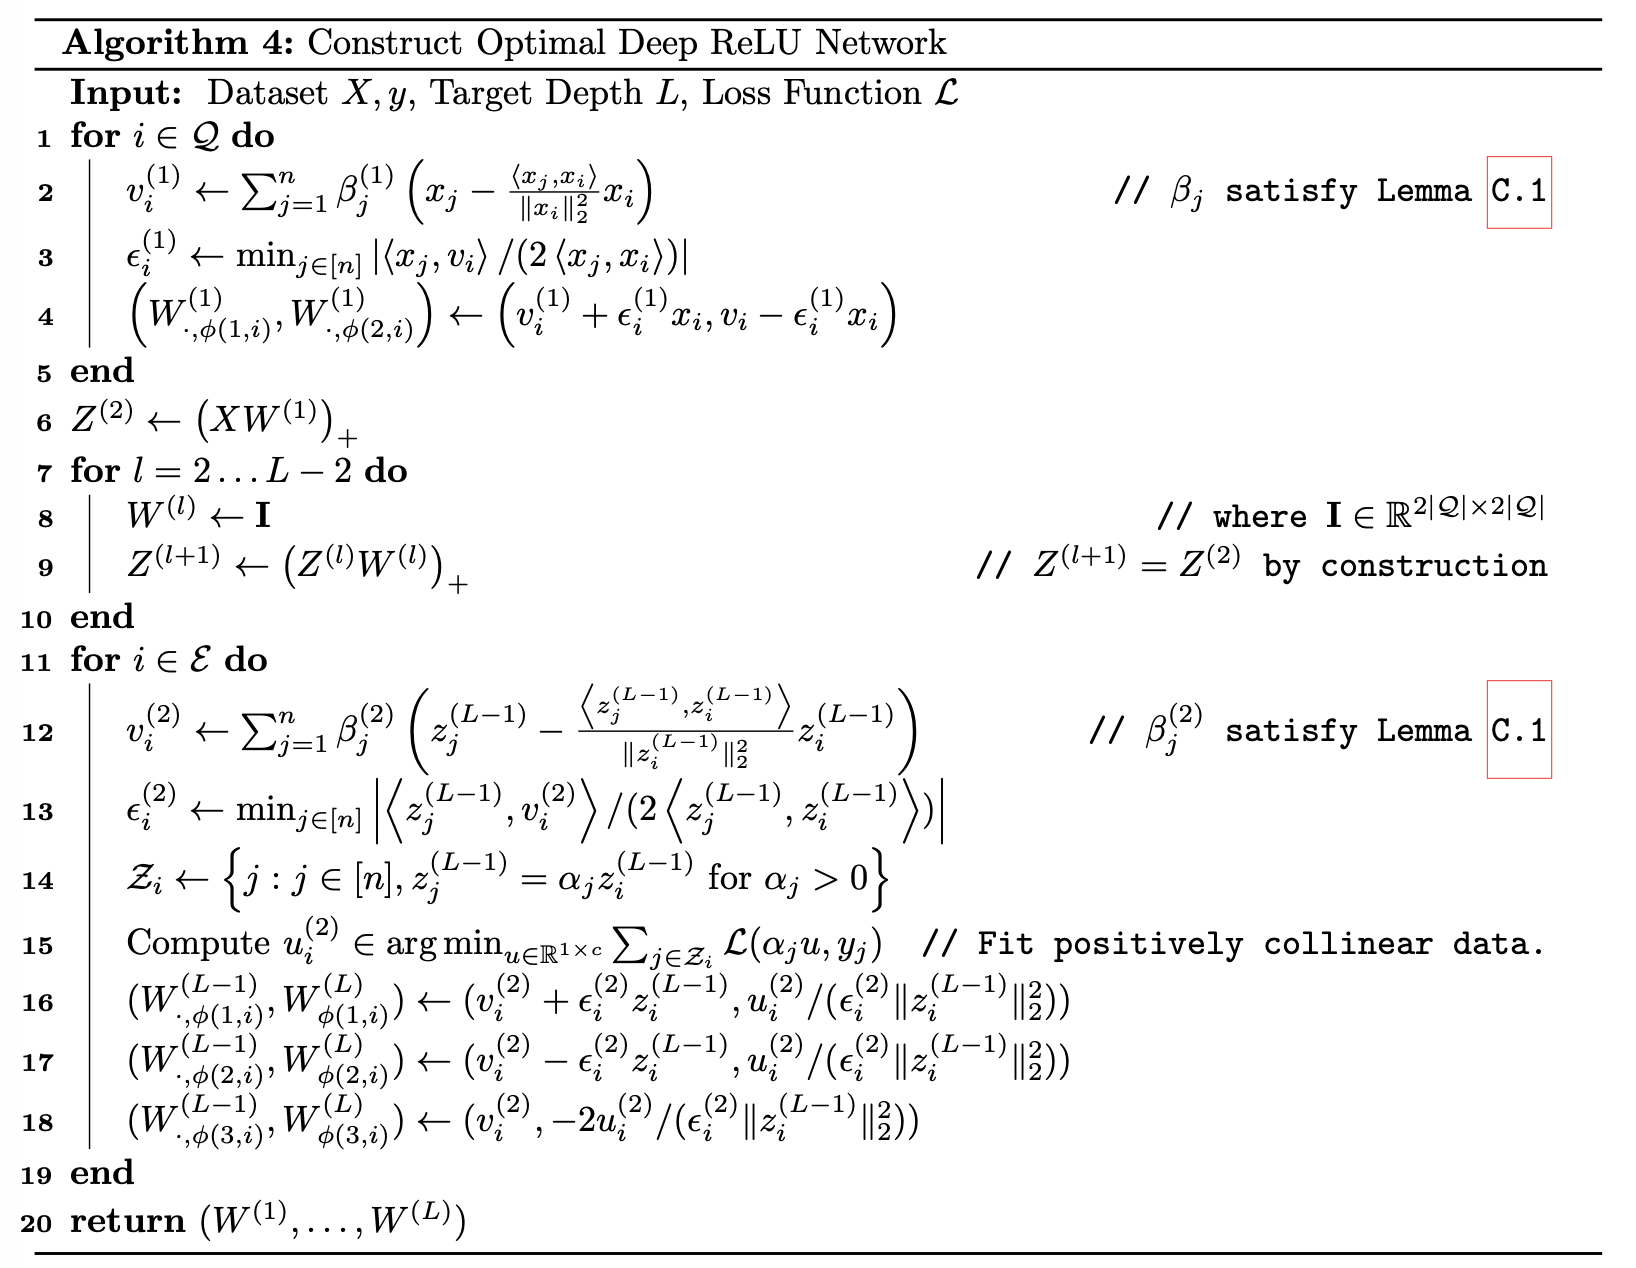
\includegraphics[width=\textwidth]{assets/l_layer_alg.png}
    \end{figure}

\end{frame}

\begin{frame}{Poly-Time Fitting: Approximations}

    We can also tackle \bad{regularized problems} in this framework:
    \pause

    \[
        \min_{W^{(1)}, W^{(2)}} \underbrace{\half \norm{\sum_{j=1}^{m_1}
                (X W^{(1)}_{\cdot, j})_+ W^{(2)}_{j} - y}_2^2}_{\text{Squared Error}}
        + \underbrace{\lambda \sum_{j=1}^m \norm{W^{(1)}_{\cdot, j}}_2^2
            + \norm{W^{(2)}_{j}}_2^2}_{\text{Weight Decay}},
    \]
    \pause

    \begin{beamercolorbox}[wd=\textwidth,sep=1em]{result}
        \textbf{Theorem}:
        If \( c = 1 \), then a model with sub-optimality
        \begin{equation*}
            \tilde{p} - p^*
            \leq 2 \lambda g(X, y)
            + \epsilon \rbr{1 + 2 \lambda \kappa\rbr{X_{\calJ}}}
        \end{equation*}
        can be computed in
        \[
            \tilde{O}\rbr{
                n_u^{3.5} (n + d)^{3.5}) \log(1 /\epsilon)
                + n_u n d \log(1 / \epsilon)
            }.
        \]
    \end{beamercolorbox}
\end{frame}

\setbeamercolor{background canvas}{bg=LightCyan}

\begin{frame}{}
    \begin{center}
        \huge 5. Big-Picture Summary
    \end{center}
\end{frame}
\setbeamercolor{background canvas}{bg=white}

\begin{frame}{Takeaways}

    \textbf{Big Idea}: we re-write optimization for \( L \)-layer ReLU networks
    as a \bad{high-dimensional} \good{convex program}.

    \pause
    \vspace{1ex}
    \horizontalrule
    \vspace{1ex}

    \textbf{Contributions}:
    \vspace{0.5ex}
    \begin{itemize}
        \item The convex reformulation is an \good{unconstrained tensor program}
              with \bad{exponential size} even in fixed dimension.

              \pause
              \vspace{1ex}

        \item Restricting the convex program to a ``representative subset''
              of ReLU activations enables \good{global optimization} in \good{poly-time}.

              \pause
              \vspace{1ex}

        \item We omit many other results, including on \good{gated ReLU networks},
              \good{optimal sets}, and deep networks with \good{regularization}.
    \end{itemize}

\end{frame}

%% bibliography
\begin{frame}[allowframebreaks]{References}
    \printbibliography[]
\end{frame}

%%!TEX root = ../main.tex

\setbeamercolor{background canvas}{bg=LightCyan}
\begin{frame}{}
    \begin{center}
        \huge Additional Projects
    \end{center}
\end{frame}
\setbeamercolor{background canvas}{bg=white}

\begin{frame}{Directional Smoothness: Summary}
    \citep{mishkin2024directional}
    Directional Smoothness and Gradient Methods: Convergence and Adaptivity.
    \good{A. Mishkin}*, A. Khaled*, Y. Wang, A. Defazio, R. M.  Gower. NeurIPS
    2024.

    \horizontalrule

    \pause
    \textbf{Big Idea}: GD is a local algorithm, so the analysis should be
    local.
    \vspace{1ex}

    \pause
    \textbf{Main Contributions}:
    \pause
    \vspace{0.5ex}
    \begin{itemize}
        \item \good{Directional Smoothness}: concrete functions \( M(x, y) \)
              that measure the Lipschitz smoothness of \( f \) between \( x \)
              and \( y \).
              \pause
              \vspace{1ex}

        \item \good{Path-Dependent Rates}: Convergence bounds for gradient descent
              that depend only on \( M(\xkk, \xk) \).
              \pause
              \vspace{1ex}

        \item \good{Adaptive Methods}: algorithms which are ``strongly adaptive''
              to the directional smoothness along the optimization path.
    \end{itemize}
\end{frame}

\begin{frame}{Level Set Teleportation: Summary}
    \citep{mishkin2025level}
    Level Set Teleportation: An Optimization Perspective. \good{A.  Mishkin},
    A. Bietti, R. M. Gower. AISTATS 2025.

    \horizontalrule
    \pause

    \textbf{Big Idea}: rigorously analyze and experimentally evaluate
    Newton-like ``teleportation'' methods \citep{zhao2022symmetry}.

    \vspace{1ex}

    \pause
    \textbf{Main Contributions}:
    \pause
    \vspace{0.5ex}
    \begin{itemize}
        \item \good{Sub-Level Set Teleportation}:
              a co-routine to accelerate optimization by maximizing the gradient
              over a sub-level set,
              \[
                  x_k^+ = \argmin_x \cbr{\norm{\grad(x)}_2 : f(x) \leq f(x_k)}.
              \]
              \pause

        \item We give a novel analysis combining \good{linear progress}
              from teleportation with sub-linear
              rates for non-strongly convex GD.

              \pause
              \vspace{1ex}

        \item We also develop \good{parameter-free algorithms} for solving
              general, non-linear sub-level set teleportation problems in
              practice.
    \end{itemize}
\end{frame}

\begin{frame}{Glocal Smoothness: Summary}
    \citep{fox2025glocal}
    Glocal Smoothness: Line Search can really help! C. Fox, \good{A.  Mishkin},
    S. Vaswani, M. Schmidt. SIOPT (\red{In Review}).

    \horizontalrule

    \pause
    \textbf{Big Question}: Can we show provable speed-ups from line-search?
    \vspace{1ex}

    \pause
    \textbf{Main Contributions}:
    \pause
    \vspace{0.5ex}
    \begin{itemize}
        \item \good{Glocal smoothness}: functions which are globally
              \( L \)-Lipschitz smooth and locally \( L^* \)-smooth
              (\( L^* \ll L \)) around minimizers.
              \pause
              \vspace{1ex}

        \item Convergence rates showing GD with exact line-search and GD with
              the Polyak step-size \good{adapt} to glocal smoothness.

              \pause
              \vspace{1ex}

        \item Extensions to \good{Nesterov acceleration}, with and without
              a backtracking line-search.
    \end{itemize}
\end{frame}

\begin{frame}{Greedy Block-Coordinate Descent: Summary}
    \citep{ramesh2023greedy}
    Greedy 2-Coordinate Updates for Equality-Constrained Optimization via Steepest
    Descent in the 1-Norm. A. V. Ramesh*, \good{A. Mishkin}*, M. Schmidt, et al.
    (\red{To Be Submitted})

    \horizontalrule
    \pause

    \textbf{Problem}: greedy rules out-perform random selection for training
    SVMs, but rates don't reflect this.

    \vspace{1ex}

    \pause
    \textbf{Main Contributions}:
    \pause
    \vspace{0.5ex}
    \begin{itemize}
        \item New analyses of \good{block-coordinate descent} for separable
              optimization problems with linear coupling constraints.
              \pause
              \vspace{1ex}

        \item \good{Single Constraint}: We prove that the GS-q rule
              \citep{tseng2009block} is equivalent to steepest descent in the
              \( \ell_1 \)-norm, leading to fast rates with \( \mu_1 \)
              dependence.

              \pause
              \vspace{1ex}

        \item \good{Multiple Constraints}: We extend the conformal vector
              framework used by \citet{tseng2009block} to obtain rates
              which improve with block-size.
    \end{itemize}
\end{frame}

\begin{frame}{Gradient Flows: Summary}
    Global Convergence of Gradient Flow on 1D Data with Sign Noise.  \good{A.
        Mishkin}, F. Bach. (\red{Ongoing})

    \horizontalrule
    \pause

    \textbf{Big Idea}: understand how ``neuron diversity'' affects convergence
    of the gradient flow for shallow ReLU networks.

    \vspace{1ex}

    \pause
    \textbf{Main Contributions}:
    \pause
    \vspace{0.5ex}
    \begin{itemize}
        \item \good{Diversity}: model neurons have different activation patterns.
              \pause
              \vspace{1ex}

        \item We find diversity is preserved for simple anti-correlated noise
              and the gradient flow is \good{globally convergent}.
              \pause
              \vspace{1ex}

        \item The gradient flow demonstrates \good{saddle-to-saddle dynamics}
              \citep{pesme2023saddle}, with saddles corresponding to model
              complexity.
              \pause
              \vspace{1ex}
    \end{itemize}

    \textbf{Remaining Extensions}:
    \pause
    \begin{enumerate}
        \item Generalize the target noise to more \bad{interesting/realistic}
              regimes (e.g. fractional Brownian motion).
    \end{enumerate}
\end{frame}

\setbeamercolor{background canvas}{bg=LightCyan}
\begin{frame}{}
    \begin{center}
        \huge Background on Convex Neural Networks
    \end{center}
\end{frame}
\setbeamercolor{background canvas}{bg=white}

\begin{frame}{Bonus: Convex Neural Networks}
    \begin{itemize}
        \item Let \( X \in \R^{n \times d} \) be a training matrix and \( y \in \R^n \)
              the targets.
              \vspace{1ex}
              \pause

        \item Let \( f_\theta : \R^n \into \R \) be a neural network with parameters
              \( \theta \).
    \end{itemize}
    \vspace{1ex}
    \pause
    The standard ERM training problem is,
    \[
        \Theta^* = \argmin_{\theta} \sum_{i=1}^n \mathcal{L}(f_\theta(x_i), y_i) + r(\theta),
    \]
    where \( \calL \) is a loss function and \( r \) is a regularizer.
    \pause
    \vspace{1ex}

    \begin{itemize}
        \item \( f_\theta \) is a \good{convex neural network} if this problem
              is convex in \( \theta \).
              \vspace{1ex}
              \pause
        \item This is distinct from \bad{input-convex} neural networks, where
              \( x \mapsto f_\theta(x) \) is convex \citep{amos2017input}.
    \end{itemize}

\end{frame}

\begin{frame}{Bonus: Brief Literature Review}
    There are multiple flavours of convex neural networks:
    \vspace{1ex}

    \begin{itemize}
        \item \citet{bengio2005convex} develop a \good{gradient-boosting algorithm}
              where the problem of adding one neuron at a time is convex.
              \pause
              \vspace{1ex}

        \item \citet{bach2017breaking} study the generalization performance of
              \good{infinite-width} two-layer neural networks (which are convex).
              \pause
              \vspace{1ex}

        \item \citet{pilanci2020convex} develop finite-width \textbf{convex
                  reformulations} for two-layer ReLU networks using \good{duality}.
              \pause
    \end{itemize}
    \vspace{1ex}

    These approaches differ primarily in how they discretize the underlying
    infinite-width neural network.

\end{frame}

\begin{frame}{Bonus: Function Space Viewpoint}
    \citet{bengio2005convex, bach2017breaking} take a function space approach:

    \begin{itemize}
        \item Let \( \sigma \) be an activation function and define
              \[
                  \calH = \cbr{h : w \in \R^d, h(x) = \sigma(x^\top w)}.
              \]
              \pause

        \item Write problem as optimization over function space \( W \):
              \[
                  \min_{w \in \calW} \cbr{\sum_{j=1}^n L\rbr{\sum_{h_i \in \calH} w_i h_i(x_j), y_j} + R(w)}.
              \]

              \pause

        \item If \( R \) is sparsity inducing, then the final network may have finite width.
    \end{itemize}

\end{frame}

\begin{frame}{Bonus: Related Work Cont.}
    \citet{bengio2005convex}: algorithm-focused approach.
    \vspace{1ex}
    \begin{itemize}
        \item Take \( R(w) = \norm{w}_1 \) and \( L(\hat y, y) = \max\cbr{0, 1 - \hat y y} \).
              \pause
              \vspace{1ex}
        \item Show that \( \text{nnz}(w^*) \leq n+1 \), meaning the final model is finite.
              \pause
              \vspace{1ex}
        \item Propose a boosting-type algorithm for iteratively adding neurons.
    \end{itemize}

\end{frame}
\begin{frame}{Bonus: Related Work Cont.}
    \citet{bach2017breaking}: analysis-focused approach.

    \begin{itemize}
        \item Handle spaces/functions properly using measure theory.
              \vspace{1ex}
              \pause
              \begin{itemize}
                  \item \( \calW \) is a space of signed measures, prediction is
                        \[
                            f(x) = \int_{\calH} h(x) dw(h)
                        \]
                        \vspace{1ex}
                        \pause

                  \item \( R \) is weighted total variation of measure \( w \).
                        \pause
                        \vspace{1ex}

                  \item Setup reduces to \citet{bengio2005convex} in finite spaces.
              \end{itemize}

              \pause
              \vspace{1ex}
        \item Guarantee that \( m^* \leq n \) using a representer theorem.
              \pause
              \vspace{1ex}

        \item Derive an incremental algorithm based on Frank-Wolfe, but incremental steps are NP-Hard
              for ReLU activations.
    \end{itemize}

\end{frame}

\begin{frame}{Bonus: Key Representer Theorem}
    \begin{theorem}[\citet{rogosinski1958moments}]
        If \( \rbr{\Omega, \calB} \) is a Borel space, \( \mu \) is a measure,
        \( g_i \), \( i \in \cbr{1, \ldots n} \) are measurable and \( \mu \)-integrable,
        then there exists measure \( \hat \mu \) with finite support at most \( n \)
        such that
        \[
            \int_\Omega g_i(\omega) d\mu(\omega) = \int_\Omega g_i(\omega) d \hat \mu(\omega)
        \]
        for all \( i \in \cbr{1,\ldots,n} \).
    \end{theorem}

    Prediction for dataset with \( n \) dimensions:
    \[
        f(x_i) = \int_{\calH} h(x_i) dw(h) = \sum_{h = 1}^m h_j(x_i) w(h_j),
    \]
    where \( m \leq n \) and \( h_j(x) = \rbr{\abr{x, w_j}}_+ \).
\end{frame}

\setbeamercolor{background canvas}{bg=LightCyan}
\begin{frame}{}
    \begin{center}
        \huge Convex Reformulations
    \end{center}
\end{frame}
\setbeamercolor{background canvas}{bg=white}

\begin{frame}{Convex Reformulations: Breaking it Down}

    \[
        \begin{aligned}
            \min_{u} & \norm{\sum_{j=1}^p D_j X (v_j - w_j) - y}_2^2 +
            \lambda \sum_{j=1}^p \norm{v_j}_2 + \norm{w_j}_2           \\
                     & \hspace{0.2em} \text{s.t. }
            v_j, w_j \in \calK_j := \cbr{w : (2D_j - I) X w \geq 0},
        \end{aligned}
    \]
    where \( \purple{D_j = \text{diag}[\mathbbm{1}(X g_j \geq 0)]} \).

    \horizontalrule

    \begin{itemize}
        \item \purple{\( D_j \) is a ReLU activation pattern induced by ``gate'' \( g_j \).}
              \pause
              \begin{itemize}
                  \item \([D_j]_{ii} = 1\) if \( \abr{x_i, g_i} \geq 0 \) and \( 0 \) otherwise.
              \end{itemize}

    \end{itemize}
    \vspace{7.3em}
\end{frame}

\begin{frame}{Convex Reformulations: Breaking it Down}

    \[
        \begin{aligned}
            \min_{u} & \norm{\sum_{j=1}^p D_j X (v_j - w_j) - y}_2^2 +
            \purple{\lambda \sum_{j=1}^p \norm{v_j}_2 + \norm{w_j}_2}  \\
                     & \hspace{0.2em} \text{s.t. }
            v_j, w_j \in \calK_j := \cbr{w : (2D_j - I) X w \geq 0}
        \end{aligned}
    \]
    where \( D_j = \text{diag}[\mathbbm{1}(X g_j \geq 0)] \).

    \horizontalrule

    \begin{itemize}
        \item \( D_j \) is a ReLU activation pattern induced by ``gate'' \( g_j \).
              \begin{itemize}
                  \item \([D_j]_{ii} = 1\) if \( \abr{x_i, g_i} \geq 0 \) and \( 0 \) otherwise.
              \end{itemize}
        \item \purple{Weight-decay regularization turns into ``group \( \ell_1 \)'' penalty.}
    \end{itemize}
    \vspace{6em}
\end{frame}

\begin{frame}{Convex Reformulations: Breaking it Down}

    \[
        \begin{aligned}
            \min_{u} & \norm{\sum_{j=1}^p D_j X (v_j - w_j) - y}_2^2 +
            \lambda \sum_{j=1}^p \norm{v_j}_2 + \norm{w_j}_2           \\
                     & \hspace{0.2em} \purple{\text{s.t. }
                v_j, w_j \in \calK_j := \cbr{w : (2D_j - I) X w \geq 0},}
        \end{aligned}
    \]
    where \( D_j = \text{diag}[\mathbbm{1}(X g_j \geq 0)] \).

    \horizontalrule

    \begin{itemize}
        \item \( D_j \) is a ReLU activation pattern induced by ``gate'' \( g_j \).
              \begin{itemize}
                  \item \([D_j]_{ii} = 1\) if \( \abr{x_i, g_i} \geq 0 \) and \( 0 \) otherwise.
              \end{itemize}
        \item Weight-decay regularization turns into ``group \( \ell_1 \)'' penalty.
        \item \purple{The constraint \( v_j \in \calK_j \) implies
                  \[
                      \rbr{X v_j}_+ = D_j X v_j.
                  \]
                  That is, \( v_j \) has the activation encoded by \( D_j \).
              }
    \end{itemize}
\end{frame}

\begin{frame}{Bonus: Explicit Solution Mapping}

    Given \( \rbr{v^*, w^*} \), an optimal non-convex ReLU network is given by

    \begin{equation*}
        \textbf{C to NC:} \quad \quad
        \begin{aligned}
            W_{1i} & = v_i^*/ \sqrt{\norm{v_i^*}}, \quad w_{2i} = \sqrt{\norm{v_i^*}}
            \\
            W_{1j} & = w_i^*/ \sqrt{\norm{w_i^*}}, \quad w_{2j} = -\sqrt{\norm{w_i^*}}.
        \end{aligned}
    \end{equation*}

    \begin{itemize}
        \item Optimal solution balances weight between layers.
    \end{itemize}

    \horizontalrule

    Given \( (W^*_{1i}, w^*_{2i}) \), an optimal convex ReLU model is

    \begin{equation*}
        \textbf{NC to C:} \quad \quad
        \begin{aligned}
            v_i & = W^*_{1i} \abs{w_{2i}}^* \quad \text{ if } w^*_{2i} \geq 0 \\
            w_i & = W^*_{1i} \abs{w_{2i}}^* \quad \text{ Otherwise.}
        \end{aligned}
    \end{equation*}

    \begin{itemize}
        \item Optimal solution combines weight from both layers.
    \end{itemize}

\end{frame}

\setbeamercolor{background canvas}{bg=LightCyan}
\begin{frame}{}
    \begin{center}
        \huge Gated ReLU Networks and Cone Decompositions
    \end{center}
\end{frame}
\setbeamercolor{background canvas}{bg=white}

\begin{frame}{Bonus: Gated ReLU Networks}

    \begin{beamercolorbox}[wd=\textwidth,sep=1em]{result}
        \textbf{Theorem 2.2} (informal): C-GReLU is equivalent to solving
        \[
            \textbf{NC-GReLU}: \min_{W_1, \alpha} \half \norm{\sum_{j=1}^p \phi_{g_j}(X, w_{j})\alpha - y}_2^2 + \frac{\lambda}{2} \sum_{j=1}^p \norm{w_{j}}_2^2 + |\alpha_j|^2,
        \]
        with the ``Gated ReLU'' \citep{fiat2019decoupling} activation function
        \[ \phi_{g}(X, u) = \text{diag}(\mathbbm{1}(Xg \geq 0)) X u, \]
        and gate vectors \( g_j \) such that
        \[
            D_j = \text{diag}[\mathbbm{1}(X g_j \geq 0).
        \]
    \end{beamercolorbox}
    \pause

    \textbf{Interpretation}: if \( u_j \not \in \calK_j \), then the activation
    must be decoupled from the linear mapping in the non-convex model.

\end{frame}

\begin{frame}{Bonus: Cone Decompositions}

    \begin{center}
        \textbf{Question}: when are Gated ReLU and ReLU networks equivalent?
    \end{center}

    \pause
    \horizontalrule

    Consider special case where \( \lambda = 0 \).

    \[
        \textbf{C-GReLU}: \min_{u} \norm{\sum_{j=1}^p D_j X u_j - y}_2^2. \hspace{11em}
    \]
    \vspace{-1em}

    \begin{center}
        \Large \red{V.S.}
    \end{center}

    \vspace{-2em}
    \[
        \begin{aligned}
            \textbf{C-ReLU}: \min_{u} & \norm{\sum_{j=1}^p D_j X (v_j - w_j) - y}_2^2. \\
                                      & \hspace{0.2em} \text{s.t. }
            v_j, w_j \in \calK_j := \cbr{w : (2D_j - I) X w \geq 0},
        \end{aligned}
    \]

\end{frame}

\begin{frame}{Bonus: Equivalent Statement}

    \red{Equiv. Question}: when does \( u_j = v_j - w_j \) for some \( v_j, w_j \in \calK_j \)?

    \pause
    \vspace{1em}

    \green{Answer}: when \( \calK_j - \calK_j = \R^d \) and a ``cone decomposition'' exists.
    \pause

    \begin{figure}[]
        \centering
        %! TEX root = ../../main.tex

%% Illustration of cone decomposition. 

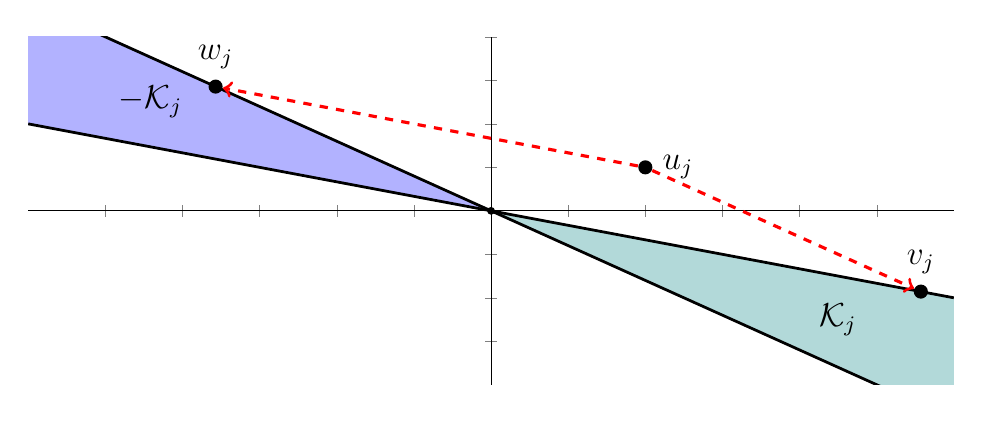
\begin{tikzpicture}[scale=1,
		declare function={
				cone_u(\x)= -\x/3;
				cone_l(\x)= -4*\x/5;
			}
	]
	\begin{axis}[width=1.1\linewidth, height=6cm,
			axis lines=center, yticklabels={,,}, xticklabels={,,},
			ymin=-4, ymax=4, ytick={-5,...,5}, ylabel=$$, x axis line style={-},
				xmin=-6, xmax=6, xtick={-5,...,5}, xlabel=$$, y axis line style={-},
		]
		\addplot[name path=cone_u, domain=-6:6, samples=100, line width=1pt]{cone_u(x)};
		\addplot[name path=cone_l, domain=-6:6, samples=200, line width=1pt]{cone_l(x)};

		% add color fill to both cones.
		\addplot fill between[
				of = cone_u and cone_l,
				split, % calculate segments
				every even segment/.style = {fill=blue, fill opacity=0.3},
				every odd segment/.style  = {fill=teal, fill opacity=0.3}
			];

		%% point labels
		% origin point
		\node[circle, fill, inner sep=1pt] at (axis cs:0,0) {};

		\node[label={0:$u_j$}, circle, fill, inner sep=1.8pt] (u) at (axis cs:2,1) {};
		\node[label={90:$v_j$}, circle, fill, inner sep=1.8pt] (v) at (axis cs:25/7+2, -25/21 - 2/3) {};
		\node[label={90:$w_j$}, circle, fill, inner sep=1.8pt] (w) at (axis cs:-25/7, 20/7) {};

		% labels
		\node[label={0:$\calK_j$}] at (axis cs:4,-2.5) {};
		\node[label={180:$-\calK_j$}] at (axis cs:-3.75,2.5) {};

		% lines
		\draw [->, dashed, draw=red, line width = 0.4mm] (u) edge (w);
		\draw [->, dashed, draw=red, line width = 0.4mm] (u) edge (v);
	\end{axis}

\end{tikzpicture}%

    \end{figure}

\end{frame}

\begin{frame}{Bonus: Basic Cone Decomposition}

    \textbf{Recall}: \( \calK_j = \cbr{w : (2 D_j - I) X w \geq 0} \).
    \pause

    \begin{itemize}
        \item This is a polyhedral cone which we rewrite as
              \[
                  \calK_j = \bigcap_{i=1}^n \cbr{w : [S_j]_{ii} \cdot \abr{x_i, w} \geq 0},
              \]
              where \( S_j = (2D_j - I) \).
    \end{itemize}

    \pause
    \horizontalrule

    \begin{beamercolorbox}[wd=\textwidth,sep=1em]{result}
        \textbf{Proposition 3.1} (informal): If \( X \) is full row-rank,
        then \( \text{aff}(\calK_j) = \R^d \) and
        \( \calK_j - \calK_j = \R^d \).
    \end{beamercolorbox}

    \vspace{1em}

    \pause
    Unfortunately, there is no extension to full-rank \( X \).

\end{frame}

\begin{frame}{Bonus: Not All Cones are Equal}

    \textbf{Alternative Idea}: show we don't need ``singular'' cones \( \calK_j \),
    \[
        \calK_j - \calK_j \subsetneq \R^d.
    \]

    \vspace{1em}
    \pause

    \begin{beamercolorbox}[wd=\textwidth,sep=1em]{result}
        \textbf{Proposition 3.2} (informal): Suppose \( \calK_j - \calK_j \subset \R^d \).
        Then, there exists \( \calK_i \) for which \( \calK_i - \calK_i = \R^d \)
        and \( \calK_j \subset \calK_i \).
    \end{beamercolorbox}

    \pause
    \vspace{1em}

    \textbf{Interpretation}: if optimal \( u^*_j \neq 0 \), then set
    \[
        u_i' = u_j^* + u_i^*.
    \]
    It is possible to show this causes no problems.

\end{frame}

\begin{frame}{Bonus: Cone Decomposition Proof Sketch}

    \textbf{Proof}: Works by iteratively constructing \( \calK_i \) s.t. \( \calK_j \subset \calK_i \).

    \pause
    \horizontalrule

    We sketch a simpler statement:

    \vspace{1em}

    \begin{beamercolorbox}[wd=\textwidth,sep=1em]{relaxation}
        \textbf{Proposition 3.2} (informal): Suppose \( \calK_j = \cbr{0} \).
        Then, there exists \( \calK_i \) for which \( \calK_i - \calK_i = \R^d \)
        and \( \calK_j \subset \calK_i \).
    \end{beamercolorbox}

\end{frame}

\begin{frame}{Bonus: Cone Decomposition Proof Sketch}
    \[
        \calK_j' = \cbr{w : [S_j]_{11} \cdot \abr{x_1, w} \geq 0}
    \]
    \begin{figure}[]
        \centering
        %! TEX root = ../../main.tex

%% Illustration of cone decomposition. 

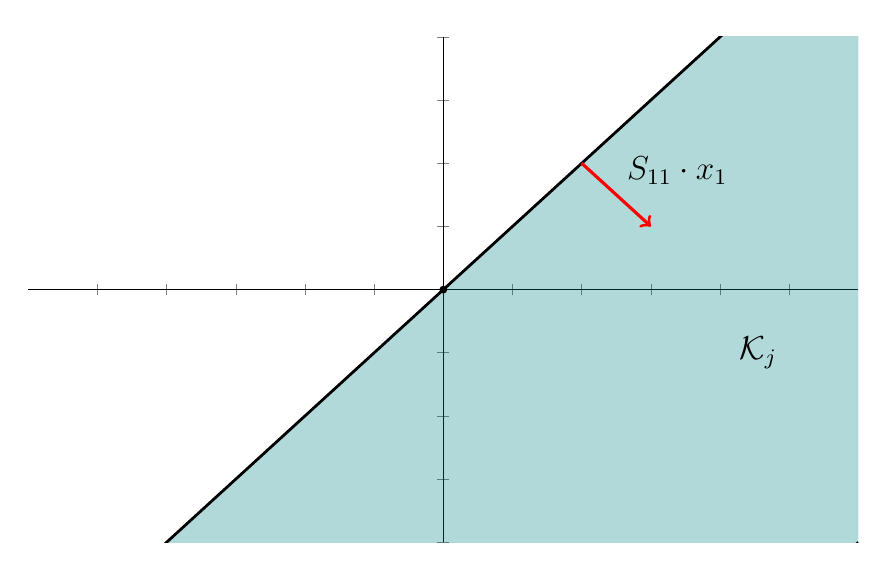
\begin{tikzpicture}[scale=1,
		declare function={
				cone_1(\x)= \x;
				cone_2(\x)= -\x;
				cone_3(\x)= -4*\x;
				bounds(\x)= \x - 10;
			}
	]
	\begin{axis}[width=\linewidth, height=8cm,
			axis lines=center, yticklabels={,,}, xticklabels={,,},
			ymin=-4, ymax=4, ytick={-5,...,5}, ylabel=$$, x axis line style={-},
				xmin=-6, xmax=6, xtick={-5,...,5}, xlabel=$$, y axis line style={-},
		]
		\addplot[name path=cone_1, domain=-6:6, samples=100, line width=1pt]{cone_1(x)};
		%\addplot[name path=cone_2, domain=-6:6, samples=200, line width=1pt]{cone_2(x)};
		%\addplot[name path=cone_3, domain=-6:6, samples=200, line width=1pt]{cone_3(x)};
		\addplot[name path=bounds, domain=-6:6, samples=100, line width=1pt]{bounds(x)};

		% add color fill to both cones.

		\addplot fill between[
				of = cone_1 and bounds,
				%split, % calculate segment
				every even segment/.style = {fill=teal, fill opacity=0.3},
			];

		%% point labels
		% origin point
		\node[circle, fill, inner sep=1pt] at (axis cs:0,0) {};

		% labels
		\node[label={0:$\calK_j$}] at (axis cs:4,-1) {};

		% lines
        \draw [->, draw=red, line width = 0.4mm] (axis cs:2,2) -- (axis cs:3,1) node[midway,above right] {$S_{11} \cdot x_1$};
		%\draw [->, draw=red, line width = 0.4mm] (axis cs:2,-2) -- (axis cs:3,-1) node[midway,below right] {$S_{22} \cdot x_2$};
		%\draw [->, draw=red, line width = 0.4mm] (axis cs:0.5,-2) -- (axis cs:-2.5,-2.75) node[pos=0.9,below right] {$S_{33} \cdot x_3$};
	\end{axis}

\end{tikzpicture}%

    \end{figure}
\end{frame}

\begin{frame}{Cone Decompositions: Proof Sketch}

    \[
        \calK_j'' = \calK_j' \cap \cbr{w : [S_j]_{22} \cdot \abr{x_2, w} \geq 0}
    \]

    \begin{figure}[]
        \centering
        %! TEX root = ../../main.tex

%% Illustration of cone decomposition. 

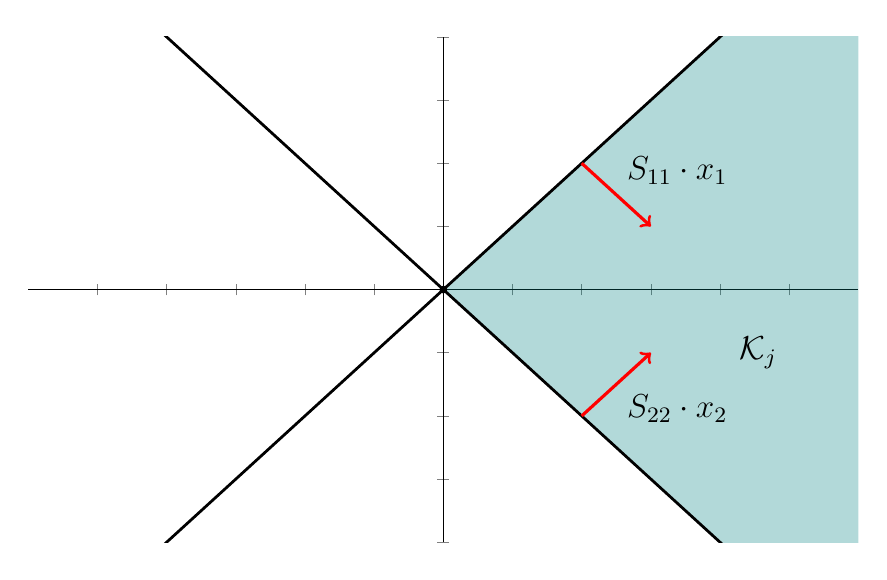
\begin{tikzpicture}[scale=1,
		declare function={
				cone_1(\x)= \x;
				cone_2(\x)= -\x;
				cone_3(\x)= -4*\x;
			}
	]
	\begin{axis}[width=\linewidth, height=8cm,
			axis lines=center, yticklabels={,,}, xticklabels={,,},
			ymin=-4, ymax=4, ytick={-5,...,5}, ylabel=$$, x axis line style={-},
				xmin=-6, xmax=6, xtick={-5,...,5}, xlabel=$$, y axis line style={-},
		]
		\addplot[name path=cone_1, domain=-6:6, samples=100, line width=1pt]{cone_1(x)};
		\addplot[name path=cone_2, domain=-6:6, samples=200, line width=1pt]{cone_2(x)};
		%\addplot[name path=cone_3, domain=-6:6, samples=200, line width=1pt]{cone_3(x)};

		% add color fill to both cones.
		\addplot fill between[
				of = cone_1 and cone_2,
				split, % calculate segments
				every even segment/.style = {fill=blue, fill opacity=0},
				every odd segment/.style  = {fill=teal, fill opacity=0.3}
			];

		%% point labels
		% origin point
		\node[circle, fill, inner sep=1pt] at (axis cs:0,0) {};

		% labels
		\node[label={0:$\calK_j$}] at (axis cs:4,-1) {};

		% lines
        \draw [->, draw=red, line width = 0.4mm] (axis cs:2,2) -- (axis cs:3,1) node[midway,above right] {$S_{11} \cdot x_1$};
		\draw [->, draw=red, line width = 0.4mm] (axis cs:2,-2) -- (axis cs:3,-1) node[midway,below right] {$S_{22} \cdot x_2$};
		%\draw [->, draw=red, line width = 0.4mm] (axis cs:0.5,-2) -- (axis cs:-2.5,-2.75) node[pos=0.9,below right] {$S_{33} \cdot x_3$};
	\end{axis}

\end{tikzpicture}%

    \end{figure}
\end{frame}

\begin{frame}{Bonus: Cone Decomposition Proof Sketch}

    \[
        \calK_j''' = \calK_j'' \cap \cbr{w : [S_j]_{33} \cdot \abr{x_3, w} \geq 0}
    \]

    \begin{figure}[]
        \centering
        %! TEX root = ../../main.tex

%% Illustration of cone decomposition. 

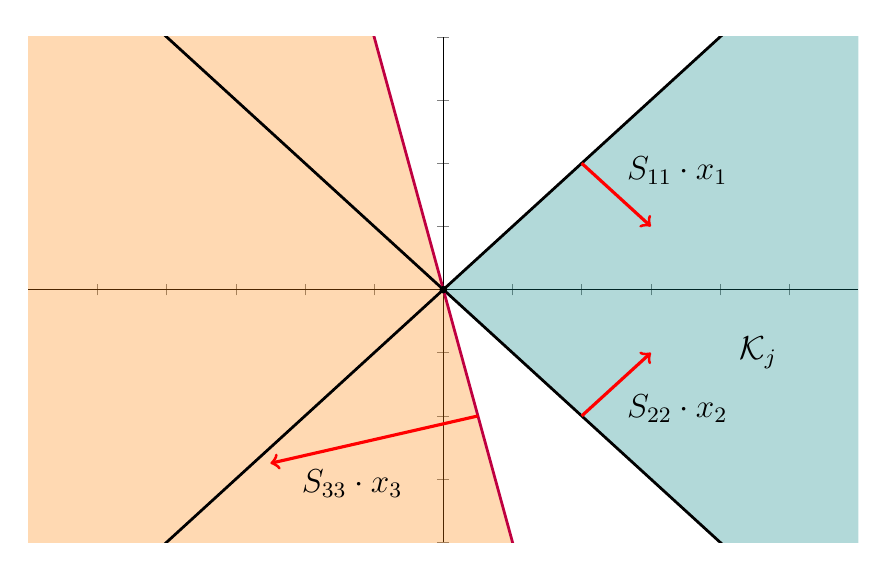
\begin{tikzpicture}[scale=1,
		declare function={
				cone_1(\x)= \x;
				cone_2(\x)= -\x;
				cone_3(\x)= -4*\x;
				bounds(\x)= -4*\x - 100;
			}
	]
	\begin{axis}[width=\linewidth, height=8cm,
			axis lines=center, yticklabels={,,}, xticklabels={,,},
			ymin=-4, ymax=4, ytick={-5,...,5}, ylabel=$$, x axis line style={-},
				xmin=-6, xmax=6, xtick={-5,...,5}, xlabel=$$, y axis line style={-},
		]
		\addplot[name path=cone_1, domain=-6:6, samples=100, line width=1pt]{cone_1(x)};
		\addplot[name path=cone_2, domain=-6:6, samples=200, line width=1pt]{cone_2(x)};
		\addplot[name path=cone_3, domain=-6:6, samples=200, line width=1pt, draw=purple]{cone_3(x)};
		\addplot[name path=bounds, domain=-6:6, samples=200, line width=1pt]{bounds(x)};

		% add color fill to both cones.
		\addplot fill between[
				of = cone_1 and cone_2,
				split, % calculate segments
				every even segment/.style = {fill=blue, fill opacity=0},
				every odd segment/.style  = {fill=teal, fill opacity=0.3}
			];

		\addplot fill between[
				of = cone_3 and bounds,
				every even segment/.style = {fill=orange, fill opacity=0.3},
			];

		%% point labels
		% origin point
		\node[circle, fill, inner sep=1pt] at (axis cs:0,0) {};

		% labels
		\node[label={0:$\calK_j$}] at (axis cs:4,-1) {};

		% lines
        \draw [->, draw=red, line width = 0.4mm] (axis cs:2,2) -- (axis cs:3,1) node[midway,above right] {$S_{11} \cdot x_1$};
		\draw [->, draw=red, line width = 0.4mm] (axis cs:2,-2) -- (axis cs:3,-1) node[midway,below right] {$S_{22} \cdot x_2$};
		\draw [->, draw=red, line width = 0.4mm] (axis cs:0.5,-2) -- (axis cs:-2.5,-2.75) node[pos=0.9,below right] {$S_{33} \cdot x_3$};
	\end{axis}

\end{tikzpicture}%

    \end{figure}
\end{frame}

\begin{frame}{Bonus: Cone Decomposition Proof Sketch}

    \[
        \tilde \calK_j''' = \calK_j'' \cap \cbr{w : -[S_j]_{33} \cdot \abr{x_3, w} \geq 0}
    \]

    \begin{figure}[]
        \centering
        %! TEX root = ../../main.tex

%% Illustration of cone decomposition. 

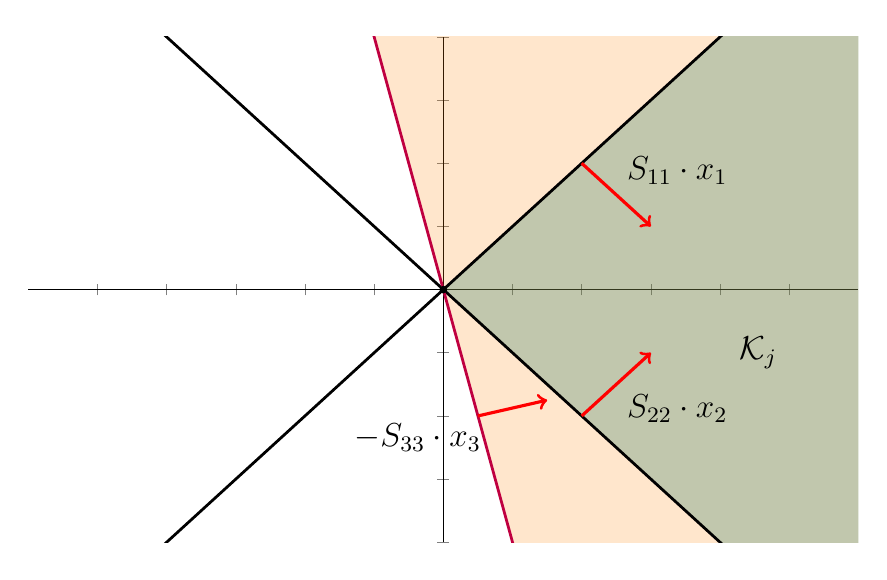
\begin{tikzpicture}[scale=1,
		declare function={
				cone_1(\x)= \x;
				cone_2(\x)= -\x;
				cone_3(\x)= -4*\x;
				bounds(\x)= -4*\x + 100;
			}
	]
	\begin{axis}[width=\linewidth, height=8cm,
			axis lines=center, yticklabels={,,}, xticklabels={,,},
			ymin=-4, ymax=4, ytick={-5,...,5}, ylabel=$$, x axis line style={-},
				xmin=-6, xmax=6, xtick={-5,...,5}, xlabel=$$, y axis line style={-},
		]
		\addplot[name path=cone_1, domain=-6:6, samples=100, line width=1pt]{cone_1(x)};
		\addplot[name path=cone_2, domain=-6:6, samples=200, line width=1pt]{cone_2(x)};
		\addplot[name path=cone_3, domain=-6:6, samples=200, line width=1pt, draw=purple]{cone_3(x)};
		\addplot[name path=bounds, domain=-6:6, samples=200, line width=1pt]{bounds(x)};

		% add color fill to both cones.
		\addplot fill between[
				of = cone_1 and cone_2,
				split, % calculate segments
				every even segment/.style = {fill=blue, fill opacity=0},
				every odd segment/.style  = {fill=teal, fill opacity=0.3}
			];

		\addplot fill between[
				of = cone_3 and bounds,
				every even segment/.style = {fill=orange, fill opacity=0.2},
			];

		%% point labels
		% origin point
		\node[circle, fill, inner sep=1pt] at (axis cs:0,0) {};

		% labels
		\node[label={0:$\calK_j$}] at (axis cs:4,-1) {};

		% lines
        \draw [->, draw=red, line width = 0.4mm] (axis cs:2,2) -- (axis cs:3,1) node[midway,above right] {$S_{11} \cdot x_1$};
		\draw [->, draw=red, line width = 0.4mm] (axis cs:2,-2) -- (axis cs:3,-1) node[midway,below right] {$S_{22} \cdot x_2$};
		\draw [->, draw=red, line width = 0.4mm] (axis cs:0.5,-2) -- (axis cs:1.5,-1.75) node[pos=0.2,below left] {$-S_{33} \cdot x_3$};
	\end{axis}

\end{tikzpicture}%

    \end{figure}
\end{frame}

\begin{frame}{Bonus: Main Cone Decomposition Result}
    \begin{itemize}
        \item The real proof is more complex, but this is the core idea.
              \vspace{0.2em}
              \begin{itemize}
                  \item Build \( \calK_i \) by switching signs of \( [S_j]_{ii} \).
                        \vspace{0.2em}
                  \item Equivalent to turning on/off activations.
              \end{itemize}
              \vspace{0.4em}

        \item Leads to our main approximation result.
    \end{itemize}

    \pause
    \horizontalrule

    \begin{beamercolorbox}[wd=\textwidth,sep=1em]{result}
        \textbf{Theorem 3.7} (informal):
        Let \( \lambda \geq 0 \) and let \( p^* \) be the optimal value of the ReLU problem.
        There exists a C-GReLU problem with minimizer \( u^* \) and optimal value \( d^* \) satisfying,
        \[
            d^* \leq p^* \leq d^* + \textcolor{Red}{2 \lambda \kappa(\tilde X_{\calJ}) \sum_{D_i \in \tilde \calD} \norm{u_i^*}_2}.
        \]
    \end{beamercolorbox}

\end{frame}

\setbeamercolor{background canvas}{bg=LightCyan}
\begin{frame}{}
    \begin{center}
        \huge Details on Optimization Algorithms
    \end{center}
\end{frame}
\setbeamercolor{background canvas}{bg=white}

\begin{frame}{Bonus: ReLU by Cone Decomposition}
    \begin{enumerate}
        \item Solve the gated ReLU problem:
              \[
                  u^* \in \argmin_{u} \norm{\sum_{j=1}^p D_j X u_j - y}_2^2 + \lambda \sum_{j=1}^p \norm{u_j}_2
              \]
              \pause
        \item Solve a cone decomposition:
              \[
                  v_j^*, w_j^* \in \argmin_{v_j, w_j} \cbr{ L(v_j, w_j) : v_j - w_j = u^*_j},
              \]
              where \( L \) is a loss function.
              \pause

        \item Compute corresponding ReLU model.
    \end{enumerate}

    \pause

    \vspace{2ex}
    \textbf{Choosing}:
    \begin{itemize}
        \item \( L(v, w) = \norm{v}_2 + \norm{w}_2 \) gives an SOCP.
              \pause

        \item \( L(v, w) = 0 \) yields a linear feasibility problem.
    \end{itemize}

\end{frame}

\begin{frame}{Bonus: R-FISTA}

    Consider ``composite'' optimization problem:
    \[
        \min_{x} f(x) + g(x),
    \]
    where \( f \) is \( L \)-smooth and \( g \) is convex.
    Smoothness implies
    \begin{equation*}
        \begin{aligned}
            f(y) & \leq Q_{\xk, 1/L}(y)                           \\
                 & = f(\xk)\! + \!\abr{\grad(\xk), y \!- \!\xk}\!
            +\! \frac{L}{2}\norm{y \!- \!\xk}_2^2.
        \end{aligned}
    \end{equation*}
    \vspace{2ex}

    \pause

    The \textbf{FISTA} algorithm minimizes \( Q_{\yk, \etak} \)
    and handles \( g \) exactly:
    \begin{align*}
        \xkk
         & = \argmin_{y} Q_{\yk, \etak}(y) + g(y)              \\
        \ykk
         & = \xkk + \frac{t_k - 1}{t_{k + 1}} \rbr{\xkk - \xk}
    \end{align*}
    where \( t_{k + 1} = (1 + \sqrt{1 + 4 t_k^2}) / 2 \).
\end{frame}

\begin{frame}{Bonus: R-FISTA Continued}
    We combine this with line-search and restarts:
    \vspace{1ex}

    \pause
    \begin{itemize}
        \item
              \textbf{Line-search}: backtrack on \( \etak \) until:
              \[
                  f(\xkk(\etak)) \leq Q_{\yk, \etak}(\xkk(\etak)),
              \]
              as proposed by \citep{beck2009fast}.
              \pause
              \vspace{1ex}
        \item
              \textbf{Restarts}: reset to \( \yk = \xk \) if
              \[ \abr{\xkk - \xk, \xkk - \yk} > 0, \]
              that is, \( \xkk \) is not a descent step
              with respect to proximal-gradient mapping
              ~\citep{odonoghue2015restarts}.

              \pause
              \vspace{1ex}
        \item And lots of other \textbf{convex tricks}...
    \end{itemize}
\end{frame}

\begin{frame}{Bonus: AL Method}
    Let \( \tilde X_i = (2 D_i - I) X \) so that
    \( v_j \in \calK_j \iff X_j v_j \geq 0 \) and define
    \[
        F(v, w) 
        = \norm{\sum_{j=1}^p D_j X (v_j - w_j) - y}_2^2 
        + \lambda \sum_{j=1}^p \norm{v_j}_2 + \norm{w_j}_2.
    \]
    Now we can form the augmented Lagrangian:
    \begin{equation}\label{eq:augmented-lagrangian}
        \begin{aligned}
            \!\!\!\!\calL_\delta & (v,\!w,\!\gamma,\!\zeta)\!:=\!(\delta / 2)\!\!\sum_{D_i \in \tilde \calD}\!\!\big[\|(\gamma_i / \delta\!-\! \tilde X_i v_i)_+\|_2^2 \\
                                 & \hspace{2em} + \|(\zeta_i / \delta - \tilde X_i w_i)_+\|_2^2 \big] + F(v,w).
        \end{aligned}
    \end{equation}
    We use the multiplier method to update the dual parameters:
    \begin{align*}
        \rbr{v_{k+1}, w_{k+1}}
                    & = \argmin_{v, w} \calL_{\delta}(v, w, \gamma_k, \zeta_k), \label{eq:al-subroutine} \\
        \gamma_{k + 1}
        = (\gamma_k & - \delta \tilde X_i v_i)_+, \quad
        \zeta_{k + 1} = (\zeta_k - \delta \tilde X_i w_i)_+. \nonumber
    \end{align*}

    \pause
    We use warm starts and propose a heuristic for \( \delta \).
\end{frame}

\setbeamercolor{background canvas}{bg=LightCyan}
\begin{frame}{}
    \begin{center}
        \huge Additional Optimization Experiments
    \end{center}
\end{frame}
\setbeamercolor{background canvas}{bg=white}

\begin{frame}{Bonus: Sub-sampling Patterns}

    \begin{figure}[t]
        \centering
        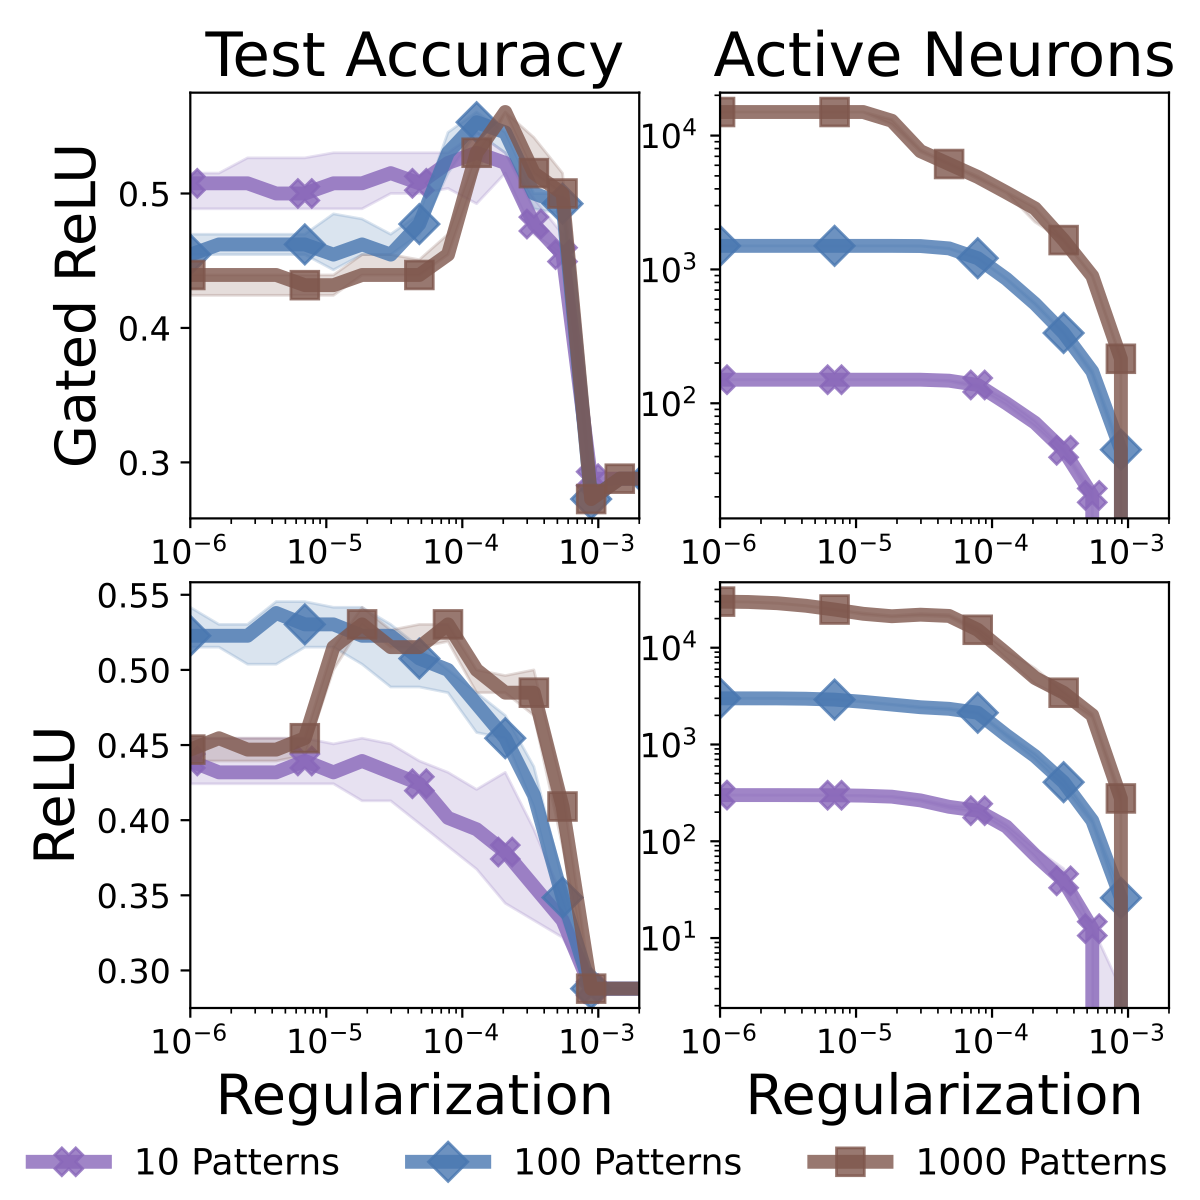
\includegraphics[width=0.6\textwidth]{assets/hp_paper.png}
    \end{figure}
    \begin{itemize}
        \item Variance induced by resampling \( \tilde \calD \) is minimal.
        \item Standard bias-variance trade-off.
    \end{itemize}
\end{frame}

\begin{frame}{Bonus: Generalization Performance}

    Generalization performance is equivalent to non-convex solvers.
    \begin{table}[t]
	\centering
	\begin{small}
		\begin{tabular}{lccc} \toprule
			\textbf{Dataset} & \textbf{Convex} & \textbf{Adam} & \textbf{SGD}  \\ \midrule
			magic            & 85.9            & \textbf{86.9} & 86.4          \\
			statlog-heart    & \textbf{83.3}   & \textbf{83.3} & 79.6          \\
            vertebral-col.   & \textbf{90.3}    & \textbf{90.3} & 88.7          \\
			cardiotocogr.    & \textbf{89.9}   & 36.5          & 88.9          \\
			abalone          & \textbf{66.2}   & 65.3          & 66.1          \\
			annealing        & 90.6            & \textbf{93.7} & 88.7          \\
			car              & 87.8            & \textbf{94.8} & 90.1          \\
			bank             & 89.8            & \textbf{90.8} & 90.5          \\
			breast-cancer    & \textbf{68.4}   & 64.9          & \textbf{68.4} \\
			page-blocks      & 94.0            & \textbf{97.1} & 96.9          \\
			contrac          & \textbf{55.1}   & 54.4          & 53.7          \\
			congressional    & 63.2            & 62.1          & \textbf{67.8} \\
			spambase         & 93.3            & \textbf{93.5} & 93.2          \\
			synthetic        & \textbf{98.3}   & 96.7          & 96.7          \\
			hill-valley      & \textbf{65.3}   & 62.8          & 55.4          \\ \bottomrule
		\end{tabular}
	\end{small}
\end{table}


\end{frame}

\begin{frame}{Bonus: Comparison to Standard Baselines}
    \setlength{\tabcolsep}{3pt} % Default value: 6pt
\begin{table}[t]
    \centering
    \begin{small}
        \begin{tabular}{lccccc} \toprule
            \small
            \textbf{Dataset} & \textbf{C-GReLU} & \textbf{C-ReLU} & \textbf{RF}   & \textbf{Linear} & \textbf{RBF}  \\ \midrule
            blood            & 79.9             & \textbf{80.5}   & 75.8          & 74.5            & 77.9          \\
            chess-krvkp      & \textbf{99.2}    & 98.6            & 98.9          & 97.2            & 98.4          \\
            conn-bench       & \textbf{90.2}    & 85.4            & 73.2          & 68.3            & 85.4          \\
            cylinder-bands   & 76.5             & \textbf{78.4}   & 77.5          & 71.6            & 71.6          \\
            fertility        & \textbf{80.0}    & \textbf{80.0}   & 75.0          & 75.0            & 75.0          \\
            heart-hung.      & \textbf{86.2}    & \textbf{86.2}   & 84.5          & 84.5            & \textbf{86.2} \\
            hill-valley      & \textbf{76.0}    & 68.6            & 57.9          & 62.0            & 70.2          \\
            ilpd-liver       & 72.4             & \textbf{74.1}   & 66.4          & 71.6            & 71.6          \\
            mammographic     & 77.6             & 78.6            & \textbf{80.7} & \textbf{80.7}   & 80.2          \\
            monks-1          & \textbf{100}     & \textbf{100}    & 95.8          & 79.2            & 83.3          \\
            musk-1           & 94.7             & \textbf{95.8}   & 92.6          & 86.3            & \textbf{95.8} \\
            ozone            & \textbf{97.6}    & \textbf{97.6}   & 97.4          & 97.2            & 97.4          \\
            pima             & 74.5             & 74.5            & \textbf{76.5} & 75.2            & 73.2          \\
            planning         & \textbf{69.4}    & 63.9            & 66.7          & 66.7            & \textbf{69.4} \\
            spambase         & 93.5             & 93.6            & \textbf{94.1} & 92.2            & 93.6          \\
            spectf           & \textbf{87.5}    & 75.0            & 68.8          & 68.8            & 68.8          \\
            statlog-german   & 74.0             & \textbf{77.5}   & 73.5          & 75.0            & 75.5          \\
            tic-tac-toe      & 99.0             & 99.0            & 99.5          & 98.4            & \textbf{100}  \\ \bottomrule
        \end{tabular}
    \end{small}
\end{table}
\setlength{\tabcolsep}{6pt}

% convex is best or ties on 24 & 38 datasets. Next best is the kernel SVM with 12 & 38 datasets.


\end{frame}

\begin{frame}{Bonus: Acceleration Ablation}
    \begin{figure}
        \centering
        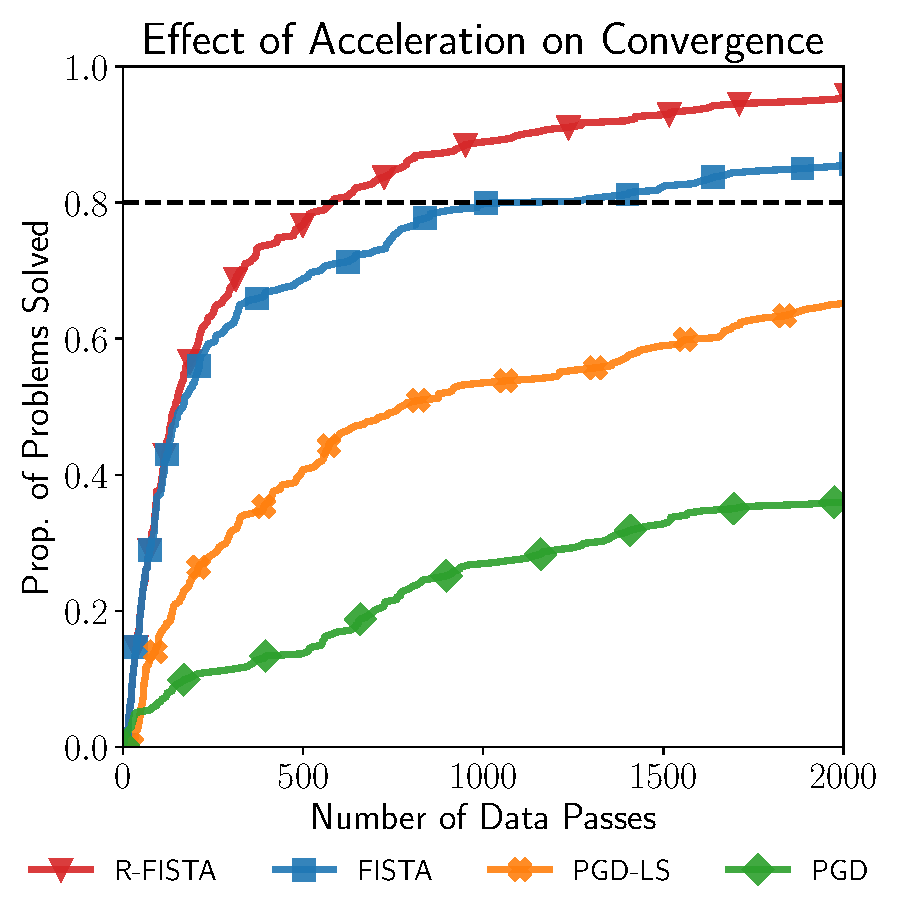
\includegraphics[width=0.75\textwidth]{assets/pp_acceleration.pdf}
    \end{figure}
\end{frame}



%%!TEX root = ../main.tex

\setbeamercolor{background canvas}{bg=LightCyan}
\begin{frame}{}
    \begin{center}
        \huge Example: Discontinuous Regularization Paths
    \end{center}
\end{frame}
\setbeamercolor{background canvas}{bg=white}

\begin{frame}{Example: Discontinuous Paths}
    Consider training a toy neural network: given \( (x_1, y_1), (x_2, y_2) \),
    \pause
    \[
        \min_{w_1} \, \half ((w_1 x_1)_+ - y_1)^2 + \half ((w_1 x_2)_+ - y_2)^2 + \lambda |w_1|.
    \]
    \pause

    \begin{center}
        %! TEX root = ../../main.tex

%% Illustration of cone decomposition. 

\begin{tikzpicture}[scale=1,
		declare function={
				loss(\x)= (4*(\x - 4)^2 + 4)*(x<=4.5) + (8*(\x - 5)^2 + 3)*(x>4.5);
			}
	]
	\begin{axis}[width=\linewidth, height=6cm,
			axis lines=center, yticklabels={,,}, xticklabels={,,},
			ymin=-2, ymax=6, ytick={-2,...,5}, ylabel=$$, x axis line style={-},
				xmin=-6, xmax=6, xtick={-5,...,5}, xlabel=$$, y axis line style={-},
		]

		\addplot[name path=loss, domain=-6:6, samples=200, line width=1pt, color=bad]{loss(x)};

		%% point labels
		% origin point
		\node[circle, fill, inner sep=1pt] at (axis cs:0,0) {};

		% active examples 
		\node[label=right:$(x_1\!\mathbin{,} y_1)$, circle, fill, inner sep=0.5mm] at (axis cs:-5,1) {};
		\node[label=right:$(x_2\!\mathbin{,} y_2)$, circle, fill, inner sep=0.5mm] at (axis cs:0.5,5) {};
	\end{axis}

\end{tikzpicture}%

    \end{center}

    \begin{center}
        \Large
        \textcolor{white}{Goal: Overcome these problems via convexification..}
    \end{center}

\end{frame}

\begin{frame}{Example: Discontinuous Paths}
    Consider training a toy ReLU network:
    \[
        \min_{w_1} \, \half ((w_1 x_1)_+ - y_1)^2 + \half ((w_1 x_2)_+ - y_2)^2 + \lambda |w_1|.
    \]

    \begin{center}
        %! TEX root = ../../main.tex

%% Illustration of cone decomposition. 

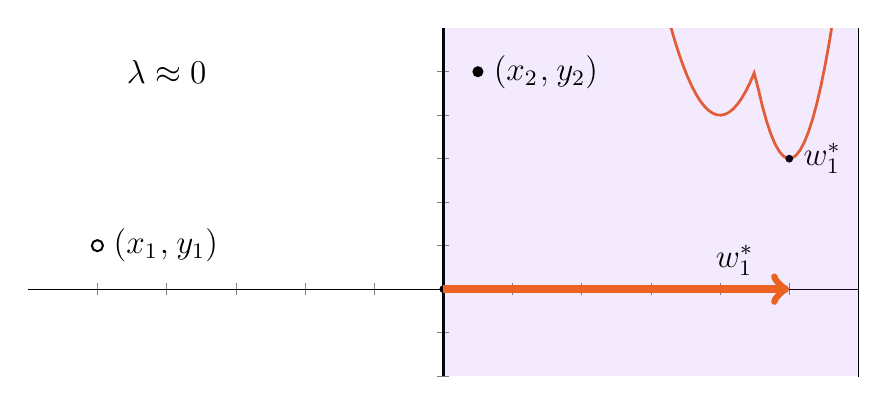
\begin{tikzpicture}[scale=1,
		declare function={
				loss(\x)= (4*(\x - 4)^2 + 4)*(x<=4.5) + (8*(\x - 5)^2 + 3)*(x>4.5);
			}
	]
	\begin{axis}[width=\linewidth, height=6cm,
			axis lines=center, yticklabels={,,}, xticklabels={,,},
			ymin=-2, ymax=6, ytick={-2,...,5}, ylabel=$$, x axis line style={-},
				xmin=-6, xmax=6, xtick={-5,...,5}, xlabel=$$, y axis line style={-},
		]

		\addplot[name path=loss, domain=-6:6, samples=200, line width=1pt, color=bad]{loss(x)};
		\node[label=right:$w_1^*$, circle, fill, inner sep=1pt] at (axis cs:5,3) {};

		\draw [name path=cone_1, solid, line width=1pt] (axis cs:0,-2) -- (axis cs:0,6);
		\draw [name path=bounds, line width=0pt] (axis cs:6,-2) -- (axis cs:6,6);
		\tikzfillbetween[of=cone_1 and bounds, on layer=ft]{good, opacity=0.1};

		%% point labels
		% origin point
		\node[circle, fill, inner sep=1pt] at (axis cs:0,0) {};

		% active examples 
		\node[label=right:$(x_1\!\mathbin{,} y_1)$, circle, draw, line width=0.25mm, inner sep=0.5mm] at (axis cs:-5,1) {};
		\node[label=right:$(x_2\!\mathbin{,} y_2)$, circle, fill, inner sep=0.5mm] at (axis cs:0.5,5) {};


		% lines
		\draw [->, draw=bad, line width = 1mm] (axis cs:0,0) -- (axis cs:5,0) node[near end,above right] {$w^*_{1}$};

		\node[] at (axis cs:-4,5) { $ \lambda \approx 0$ };
	\end{axis}

\end{tikzpicture}%

    \end{center}

    \begin{center}
        \Large
        \textcolor{white}{Goal: Overcome these problems via convexification..}
    \end{center}

\end{frame}

\begin{frame}{Example: Discontinuous Paths}
    Consider training a toy neural network:
    \[
        \min_{w_1} \, \half ((w_1 x_1)_+ - y_1)^2 + \half ((w_1 x_2)_+ - y_2)^2 + \lambda |w_1|.
    \]

    \begin{center}
        %! TEX root = ../../main.tex

%% Illustration of cone decomposition. 

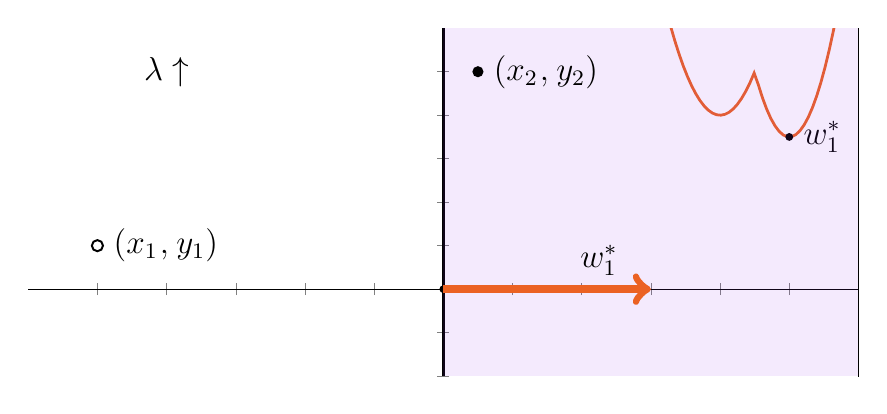
\begin{tikzpicture}[scale=1,
		declare function={
				loss(\x)= (4*(\x - 4)^2 + 4)*(x<=4.5) + (6*(\x - 5)^2 + 3.5)*(x>4.5);
			}
	]
	\begin{axis}[width=\linewidth, height=6cm,
			axis lines=center, yticklabels={,,}, xticklabels={,,},
			ymin=-2, ymax=6, ytick={-2,...,5}, ylabel=$$, x axis line style={-},
				xmin=-6, xmax=6, xtick={-5,...,5}, xlabel=$$, y axis line style={-},
		]

		\addplot[name path=loss, domain=-6:6, samples=200, line width=1pt, color=bad]{loss(x)};
		\node[label=right:$w_1^*$, circle, fill, inner sep=1pt] at (axis cs:5,3.5) {};

		\draw [name path=cone_1, solid, line width=1pt] (axis cs:0,-2) -- (axis cs:0,6);
		\draw [name path=bounds, line width=0pt] (axis cs:6,-2) -- (axis cs:6,6);
		\tikzfillbetween[of=cone_1 and bounds, on layer=ft]{good, opacity=0.1};

		%% point labels
		% origin point
		\node[circle, fill, inner sep=1pt] at (axis cs:0,0) {};

		% active examples 
		\node[label=right:$(x_1\!\mathbin{,} y_1)$, circle, draw, line width=0.25mm, inner sep=0.5mm] at (axis cs:-5,1) {};
		\node[label=right:$(x_2\!\mathbin{,} y_2)$, circle, fill, inner sep=0.5mm] at (axis cs:0.5,5) {};


		% lines
		\draw [->, draw=bad, line width = 1mm] (axis cs:0,0) -- (axis cs:3,0) node[near end,above] {$w^*_{1}$};

        \node[] at (axis cs:-4,5) { $ \lambda \uparrow $ };
	\end{axis}

\end{tikzpicture}%

    \end{center}

    \begin{center}
        \Large
        \textcolor{white}{Goal: Overcome these problems via convexification..}
    \end{center}

\end{frame}

\begin{frame}{Example: Discontinuous Paths}
    Consider training a toy neural network:
    \[
        \min_{w_1} \, \half ((w_1 x_1)_+ - y_1)^2 + \half ((w_1 x_2)_+ - y_2)^2 + \lambda |w_1|.
    \]

    \begin{center}
        %! TEX root = ../../main.tex

%% Illustration of cone decomposition. 

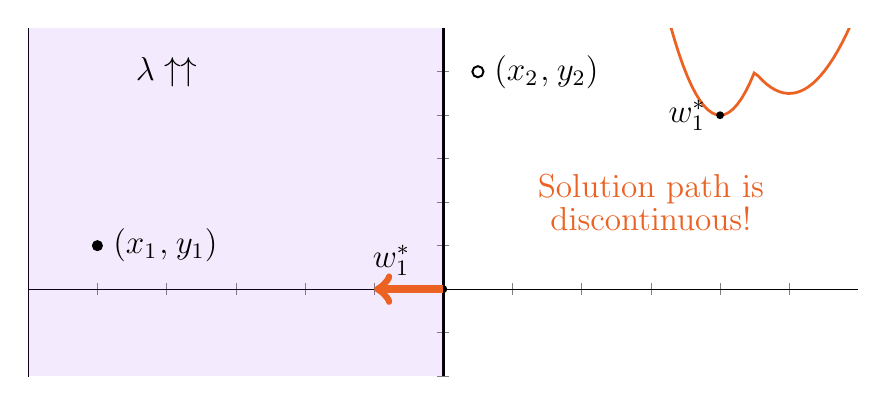
\begin{tikzpicture}[scale=1,
		declare function={
				loss(\x)= (4*(\x - 4)^2 + 4)*(x<=4.5) + (2*(\x - 5)^2 + 4.5)*(x>4.5);
			}
	]
	\begin{axis}[width=\linewidth, height=6cm,
			axis lines=center, yticklabels={,,}, xticklabels={,,},
			ymin=-2, ymax=6, ytick={-2,...,5}, ylabel=$$, x axis line style={-},
				xmin=-6, xmax=6, xtick={-5,...,5}, xlabel=$$, y axis line style={-},
		]
		\addplot[name path=loss, domain=-6:6, samples=200, line width=1pt, color=bad]{loss(x)};
		\node[label=left:$w_1^*$, circle, fill, inner sep=1pt] at (axis cs:4,4) {};

		\draw [name path=cone_1, solid, line width=1pt] (axis cs:0,-2) -- (axis cs:0,6);
		\draw [name path=bounds, line width=0pt] (axis cs:-6,-2) -- (axis cs:-6,6);
		\tikzfillbetween[of=cone_1 and bounds, on layer=ft]{good, opacity=0.1};

		%% point labels
		% origin point
		\node[circle, fill, inner sep=1pt] at (axis cs:0,0) {};

		% active examples 
		\node[label=right:$(x_1\!\mathbin{,} y_1)$, circle, fill, inner sep=0.5mm] at (axis cs:-5,1) {};
		\node[label=right:$(x_2\!\mathbin{,} y_2)$, circle, draw, line width=0.25mm, inner sep=0.5mm] at (axis cs:0.5,5) {};


		% lines
		\draw [->, draw=bad, line width = 1mm] (axis cs:0,0) -- (axis cs:-1,0) node[near end,above] {$w^*_{1}$};

		\node[] at (axis cs:-4,5) { $ \lambda \uparrow \uparrow$ };
    \node[text width=13em, text centered] at (axis cs:3,2) { \bad{Solution path} \bad{is discontinuous!} };
	\end{axis}

\end{tikzpicture}%

    \end{center}

    \pause

    \begin{center}
        \Large
        \good{Goal}: Overcome these problems via convexification.
    \end{center}

\end{frame}

\setbeamercolor{background canvas}{bg=LightCyan}
\begin{frame}{}
    \begin{center}
        \huge Optimal Sets
    \end{center}
\end{frame}
\setbeamercolor{background canvas}{bg=white}

\begin{frame}{Bonus: C-ReLU Optimality Conditions}

    We form the Lagrangian for the convex reformulation:

    \begin{equation*}
        \begin{aligned}
            \calL(v, w, \rho^{+}, \rho^{-})
             & = \half \norm{\sum_{D_i \in \tilde \calD} D_i X (v_i - w_i) - y}_2^2
            + \lambda\sum_{D_i \in \tilde \calD}\norm{v_i}_2 + \norm{w_i}_2                  \\
             & \quad \quad - \sum_{D_i \tilde \calD} \sbr{\abr{\tilde{X_i}^\top \rho^{-}, w}
                - \abr{\tilde{X_i}^\top \rho^{+}, v}},
        \end{aligned}
    \end{equation*}

    where \( \tilde X_{i} = (2D_i - I) \).

    \pause
    \horizontalrule

    The \good{KKT conditions} are necessary and sufficient for optimality:\pause

    \vspace{1ex}
    \begin{itemize}
        \item Stationary Lagrangian:
              \[
                  \underbrace{X^\top D_i (\hat y - y) - \tilde{X_i}^\top \ri^{+}}_{q_i^+} \in \partial \lambda \norm{v_i}_2.
              \]
              \pause
              \begin{itemize}
                  \normalsize
                  \item It turns out each \( q_i^+ \) is \textbf{unique} WLOG!
              \end{itemize}
    \end{itemize}

\end{frame}

\begin{frame}{Bonus: Characterizing the Optimal Set}

    \textbf{Facts}: let \( (\theta, \rho) \) be primal dual optimal. \pause
    \begin{itemize}
        \item Model fit \( \hat y \) is \blue{constant} over optimal set \( \solfn(\lambda) \). \pause
        \item Implies correlation \( X^\top D_i (y - \hat y) \) is \blue{constant} over \( \solfn(\lambda) \). \pause
        \item We may assume \( \rho \) is \blue{unique} (e.g. min-norm dual solution).
    \end{itemize}

    \pause
    \horizontalrule

    \textbf{Non-zero Blocks}:
    \begin{itemize}
        \item Suppose \( \theta_i \neq 0 \).
              \pause
        \item Then \( \nabla \norm{\theta_i}_2 = s_\bi = \lambda \theta_i / \norm{\theta_i}_2 \).
              \pause
        \item Rearranging stationarity implies \( \exists \alpha_\bi > 0 \):
              \[
                  \theta_i = \blue{\alpha_\bi} \underbrace{\sbr{X^\top D_i (y - \hat y) - \tilde X_i \ri}}_{q_i}.
              \]
              \pause
        \item Every solution is a non-negative multiple of these \( q_i \) vectors.
    \end{itemize}

\end{frame}

\begin{frame}{Bonus: Explicit Optimal Set}
    We gave a characterization of \( \solfn(\lambda) \) that depends on
    \[
        \calS_\lambda
        = \cbr{\bi \in [2p] : \exists \theta \in \solfn(\lambda), \
            \theta_i \neq 0}.
    \]

    Alternative expression involves additional linear constraints.

    \pause
    \horizontalrule

    \begin{equation*}
        \begin{aligned}
            \solfn(\lambda) =
            \big\{ & \theta  :
            \forall \, \bi  \in  \equi,
            \theta_i =  \alpha_\bi q_i, \alpha_\bi \geq 0, \,           \\
                   & \quad \forall \, j \in [2p] \setminus \equi,
            \theta_{j} = 0, \, \sum_{i=1}^{2p} D_i X \theta_i = \hat y, \\
                   & \quad \forall \, i \in [2p],
            \tilde X_i \theta_i \geq 0, \abr{\rho, \tilde X_i \theta_i } = 0.
            \big\}
        \end{aligned}
    \end{equation*}

    \pause

    More complex, but also \textbf{explicit}.

\end{frame}

\begin{frame}{Bonus: Solution Mapping for C-ReLU}

    Given \( \rbr{v^*, w^*} \), an optimal non-convex ReLU network is given by

    \begin{equation*}
        \textbf{C to NC:} \quad \quad
        \begin{aligned}
            W_{1i} & = v_i^*/ \sqrt{\norm{v_i^*}}, \quad w_{2i} = \sqrt{\norm{v_i^*}}
            \\
            W_{1j} & = w_i^*/ \sqrt{\norm{w_i^*}}, \quad w_{2j} = -\sqrt{\norm{w_i^*}}.
        \end{aligned}
    \end{equation*}

    \pause
    \vspace{3ex}
    \begin{itemize}
        \item Optimal convex weights satisfy \( v_i^* = \alpha_i q_i \)
              so that
              \[
                  \norm{v_i^*}_2 = \alpha_i \norm{q_i}_2 = \alpha_i \lambda.
              \]
    \end{itemize}

    \pause
    \horizontalrule

    Recall structure of \textbf{non-convex optima}:

    \begin{equation*}
        \begin{aligned}
            \hspace{-0.5em} \calO_\lambda  = \,
            \big\{
             & (W_1,  w_2) :
            \, f_{W_1, w_2}(X)  =  \hat y,                       \\
             & \forall \, \bi  \in  \calS_\lambda,
            W_{1i} = (\sfrac{\alpha_{i}}{\lambda})^{\sfrac{1}{2}} q_i,
            w_{2i} = (\alpha_i \lambda)^{\sfrac{1}{2}},
            \alpha_i \geq 0                                      \\
             & \forall \, \bi  \in [2p] \setminus \calS_\lambda,
            W_{1i} = 0, \, w_{2i} = 0
            \big\}.
        \end{aligned}
    \end{equation*}

\end{frame}

\setbeamercolor{background canvas}{bg=LightCyan}
\begin{frame}{}
    \begin{center}
        \huge Optimal Pruning
    \end{center}
\end{frame}
\setbeamercolor{background canvas}{bg=white}

\begin{frame}{Optimal Pruning: the Polytope of Solutions}

    \begin{columns}
        \begin{column}{0.5\textwidth}

            \begin{equation*}
                \begin{aligned}
                     & \solfn(\lambda) =
                    \big\{ \theta  : \sum_{i=1}^{2p} D_i X \theta_i = \hat y,      \\
                     & \hspace{5em} \forall \, \bi  \in  \calS_\lambda,
                    \theta_i =  \alpha_\bi q_i, \alpha_\bi \geq 0, \,              \\
                     & \hspace{5em} \forall \, j \in [2p] \setminus \calS_\lambda,
                    \theta_{j} = 0
                    \big\}
                \end{aligned}
            \end{equation*}

            \pause
            The C-ReLU optimal set is a \good{convex polytope}!

        \end{column}
        \begin{column}{0.5\textwidth}
            \pause
            \begin{figure}[c]
                \centering
                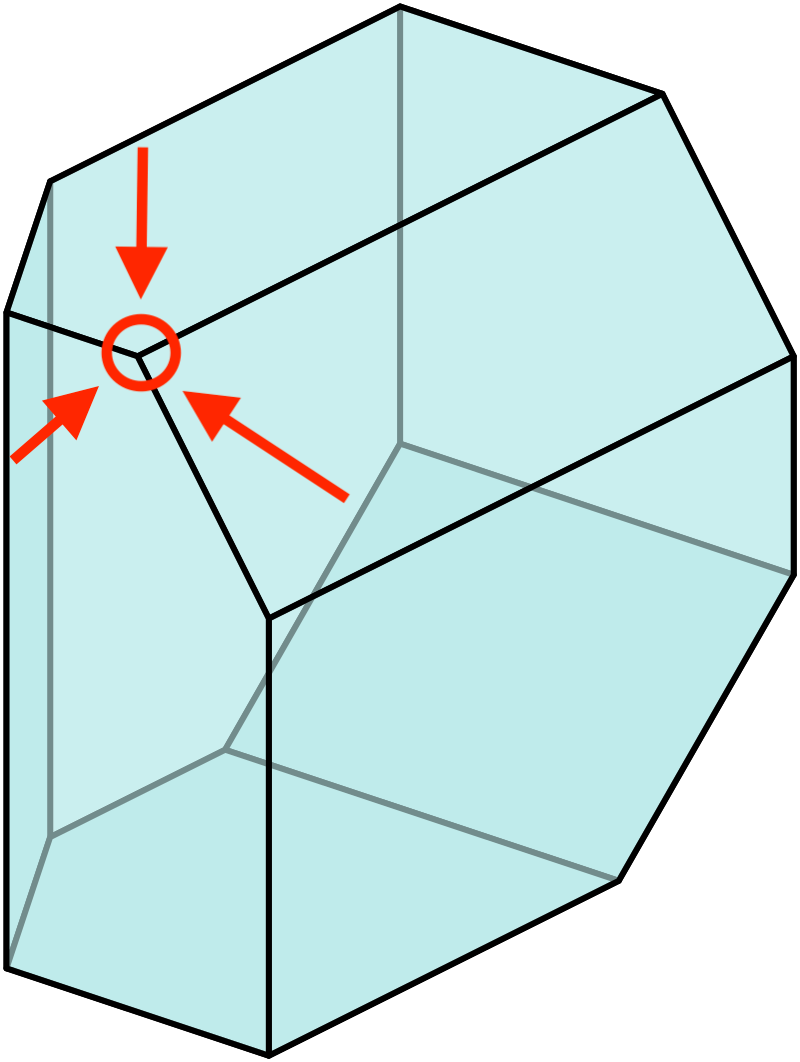
\includegraphics[width=0.8\textwidth]{assets/polytope.png}
            \end{figure}
        \end{column}
    \end{columns}

\end{frame}

\begin{frame}{Optimal Pruning: Vertices}

    \begin{enumerate}
        \item
              Stack the \( q_i \) vectors into a matrix \( Q =
              \begin{bmatrix}
                  \vert &        & \vert  \\
                  q_1   & \cdots & q_{2p} \\
                  \vert &        & \vert  \\
              \end{bmatrix}.
              \)

              \pause
        \item
              The C-ReLU Optimal Set in \( \alpha \) space is then,
              \begin{equation}
                  \begin{aligned}
                      \solfn(\lambda) & =
                      Q_{\calS_\lambda} \big\{ \alpha \succeq 0  :
                      \sum_{i \in \calS_\lambda} (D_i X q_i) \alpha_i = \hat y,
                      \big\}                                                       \\
                                      & = Q_{\calS_\lambda} \calP_{\calS_\lambda}.
                  \end{aligned}
              \end{equation}

              \pause

        \item \( \bar \alpha \in \calP_{\calS_\lambda} \) is a \good{vertex}
              iff \( \cbr{D_i X q_i}_{\bar \alpha_i \neq 0} \) are linearly independent.
    \end{enumerate}

    \pause
    \horizontalrule

    {\large Are these vertices \good{special} in some way?}

\end{frame}

\begin{frame}{Optimal Pruning: Minimal Models}
    \textbf{Definition}: An optimal C-ReLU model \( \theta^* \) is minimal if
    there does not exist another optimal model \( \theta' \) with \bad{strictly
        smaller support}.

    \pause
    \begin{itemize}
        \item \bad{NC-ReLU}: minimal \( \iff \) \good{sparsest} (neuron-wise) model.
    \end{itemize}

    \vspace{3ex}
    \pause

    \begin{beamercolorbox}[wd=\textwidth,sep=1em]{result}
        \textbf{Proposition 3.2} (informal):
        For \( \lambda > 0 \), \( \theta \in \solfn(\lambda) \) is \good{minimal}
        iff
        the vectors \( \cbr{D_i X q_i}_{\alpha_i \neq 0} \)
        are linearly independent.
    \end{beamercolorbox}

    \pause

    \begin{itemize}
        \item \bad{NC-ReLU}: minimal if \( (X W_{1i})_+ \) are linearly independent.
    \end{itemize}

    \vspace{1ex}
    \pause

    \textbf{Our Results}:
    \begin{enumerate}
        \item We prove vertices of \( \solfn(\lambda) \) are minimal models.
              \pause
        \item There are at most \( n \) neurons in a minimal model.
              \pause
        \item We give a poly-time algorithm for computing minimal models
              starting from any model \( \theta \).
    \end{enumerate}

\end{frame}

\begin{frame}{Bonus: Optimal Pruning Pseudo-code}
    \begin{algorithm}[H]
        \caption{Pruning solutions}
        \begin{algorithmic}
            \STATE {\bfseries Input:} data matrix \( X \), solution \( \theta \).
            \STATE \( k \gets 0 \).
            \STATE \( \theta^k \gets \theta \).
            \WHILE {\( \exists \beta \neq 0 \) s.t. \( \sum_{\bi \in \act(\theta^k)} \beta_\bi D_i X \theta_i^k = 0 \)}
            \STATE \( \bi^k \gets \argmax_{\bi} \cbr{|\beta_\bi| : \bi \in \act(\theta^k)}  \)
            \STATE \( t^k \gets 1/|\beta_{\bi^k}| \)
            \STATE \( \theta^{k+1} \gets \theta^k (1 - t^k \beta_\bi) \)
            \STATE \( k \gets k + 1 \)
            \ENDWHILE
            \STATE {\bfseries Output:} final weights \( \theta^k \)
        \end{algorithmic}
    \end{algorithm}

    \pause

    Let \( r = \text{rank}(X) \). Complexity to compute a minimal model:

    \[ O\rbr{d^3 r^3 (\frac{n}{r})^{3r} + \blue{(n^3 + nd) r (\frac{n}{r})^r}}. \]

\end{frame}

\begin{frame}{Bonus: Complexity of Pruning}

    \begin{algorithm}[H]
        \caption{Pruning solutions}
        \begin{algorithmic}
            \STATE {\bfseries Input:} data matrix \( X \), solution \( \theta \).
            \STATE \( k \gets 0 \), \( \theta^k \gets \theta \).
            \WHILE {\( \exists \beta \neq 0 \) s.t. \( \sum_{\bi \in \act(\theta^k)} \beta_\bi D_i X \theta_i^k = 0 \)}
            \STATE \( \vdots \)
            \ENDWHILE
            \STATE {\bfseries Output:} final weights \( \theta^k \)
        \end{algorithmic}
    \end{algorithm}

    \begin{itemize}
        \item Computing \( a_i = D_i X \theta_i^0 \) for every neuron: \( O(ndp)  \)
              \pause
              \vspace{1ex}
        \item Checking for linear dependence: at most \( 2p \) times, do
              \pause
              \vspace{1ex}
              \begin{itemize}
                  \item check (at most) \( n+1 \) \( a_i \) vectors for linearly dependence.
                        \pause
                  \item Form matrix \( A \) and take SVD to compute null space: \( O(n^3) \).
                        \pause
                  \item Prune neuron: update at most \( n \) weights.
                        \pause
                        \vspace{1ex}
              \end{itemize}
    \end{itemize}
    Total complexity: \( O(ndp + n^3 p) \).

\end{frame}

\begin{frame}{Bonus: Sub-Optimal Pruning}

    \begin{algorithm}[H]
        \caption{Pruning solutions}
        \begin{algorithmic}
            \STATE {\bfseries Input:} data matrix \( X \), solution \( \theta \).
            \STATE \( k \gets 0 \).
            \STATE \( \theta^k \gets \theta \).
            \WHILE {\( \exists \beta \neq 0 \) s.t. \( \bad{\sum_{\bi \in \act(\theta^k)} \beta_\bi D_i X \theta_i^k = 0} \)}
            \STATE \( \bi^k \gets \argmax_{\bi} \cbr{|\beta_\bi| : \bi \in \act(\theta^k)}  \)
            \STATE \( t^k \gets 1/|\beta_{\bi^k}| \)
            \STATE \( \theta^{k+1} \gets \theta^k (1 - t^k \beta_\bi) \)
            \STATE \( k \gets k + 1 \)
            \ENDWHILE
            \STATE {\bfseries Output:} final weights \( \theta^k \)
        \end{algorithmic}
    \end{algorithm}

    \pause
    Approximate with least-squares fit:
    \[
        \hat{\beta} \in \argmin_{\beta} \half \norm{\sum_{\bi \in \act(\theta^k) \setminus j} \beta_\bi D_i X \theta_i^k - D_j X \theta_j}_2^2
    \]
\end{frame}

\begin{frame}{Bonus: Sub-optimal Pruning}
    Approximate with least-squares fit:
    \[
        \hat \beta \in \argmin_{\beta} \half \norm{\sum_{\bi \in \act(\theta^k) \setminus j} \beta_\bi D_i X \theta_i^k - D_j X \theta_j}_2^2
    \]

    \horizontalrule

    \begin{itemize}
        \item Algorithm is just structured pruning with a \good{correction step}!
              \pause
        \item We use \good{existing literature} for structured pruning to select \( j \).
              \pause
        \item \bad{Brute-force search} works best:
              \[
                  \argmin_{j} \cbr{\min_{\beta} \half \norm{\sum_{\bi \in \act(\theta^k) \setminus j} \beta_\bi D_i X \theta_i^k - D_j X \theta_j}_2^2}
              \]
    \end{itemize}

\end{frame}

\begin{frame}{Neuron Pruning: Performance on CIFAR-10}
    \begin{figure}[t]
        \centering
        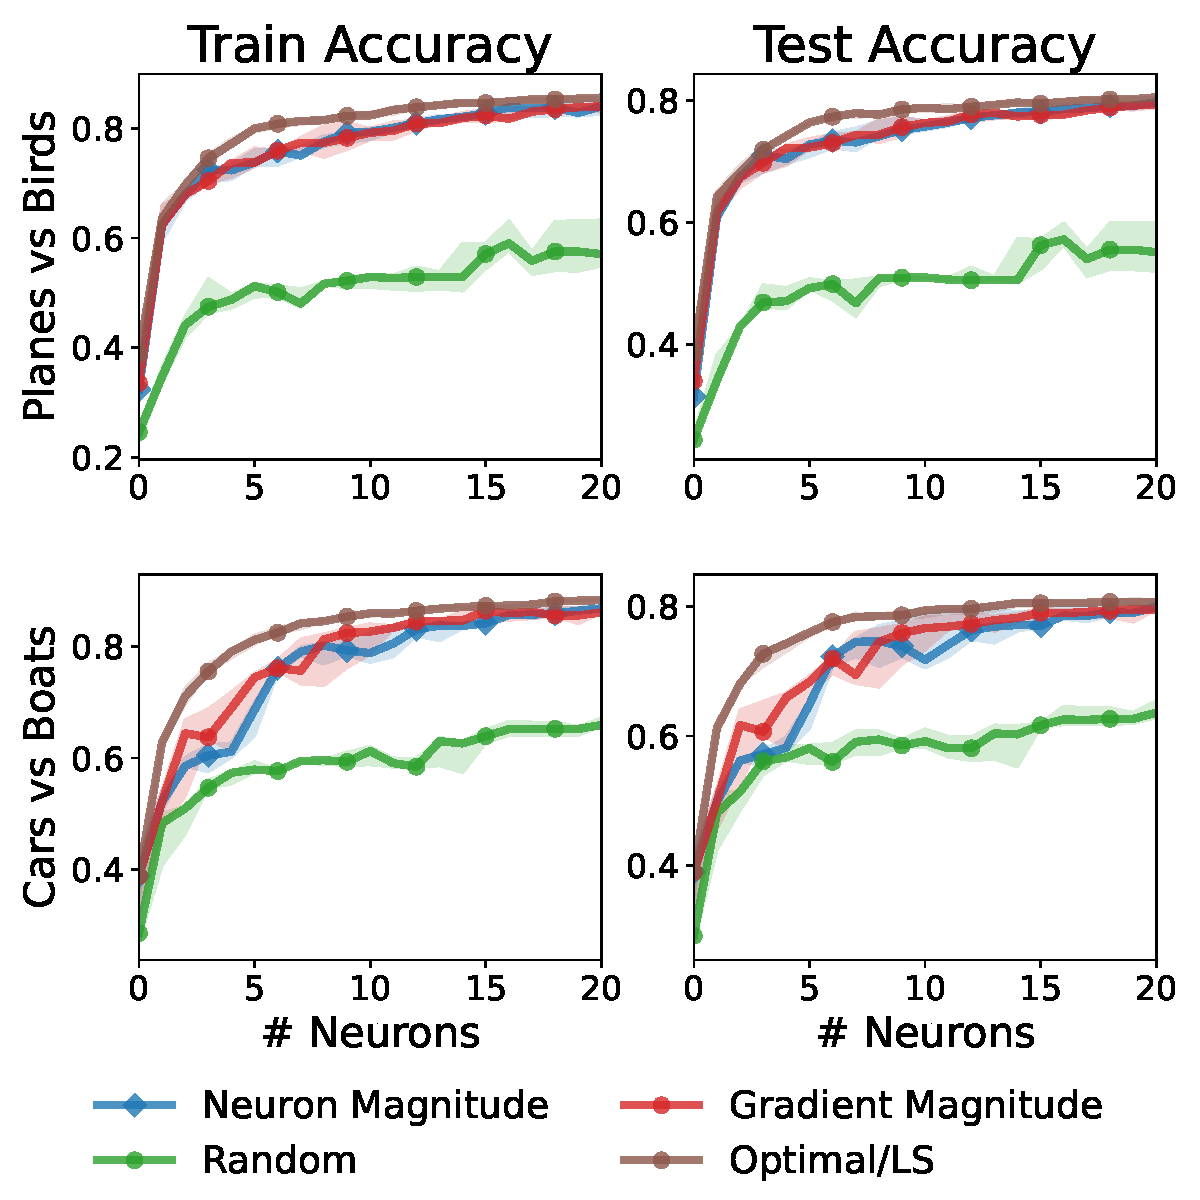
\includegraphics[width=0.75\textwidth]{assets/prune_cifar.pdf}
    \end{figure}
\end{frame}

\setbeamercolor{background canvas}{bg=LightCyan}
\begin{frame}{}
    \begin{center}
        \huge Convex Reformulations of Deep ReLU Networks
    \end{center}
\end{frame}
\setbeamercolor{background canvas}{bg=white}

\begin{frame}{Deep Reformulations: Setup}

    \begin{itemize}
        \item Let \( X^{(l)} \) and \( T^{(l)} \) be tensors of order
              \( l+1 \) indexed by \( i_0, \ldots, i_{l} \).

              \vspace{1ex}

        \item We assume  \( R^{(l)}_{i_1, \ldots, i_{l-1}} \in \R^{n \times d_0} \) and \( T^{(l)}_{i_1, \ldots, i_{l-1}} \in \R^{d_0 \times d_{l}} \).

    \end{itemize}

    \horizontalrule

    We equip these tensors with the reduction product
    \begin{equation*}\label{eq:reduction-prod}
        R^{(l)} \odot T^{(l)}
        = \sum_{i_1, \ldots, i_{l-1}} R^{(l)}_{i_1, \ldots, i_{l-1}}
        T^{(l)}_{i_1, \ldots, i_{l-1}},
    \end{equation*}

    \begin{itemize}
        \item This sums over the product of all the matrix slices
              \( R^{(l)}_{i_1, \ldots, i_{l-1}} \) and
              \( T^{(l)}_{i_1, \ldots, i_{l-1}} \).
    \end{itemize}

\end{frame}

\begin{frame}{Deep Reformulations: Recursive Patterns}
    \begin{itemize}
        \item Let \( \calD^{(1)}_X \) be the set of achievable
              ReLU patterns in the first layer.

        \item Let \( X^{(1)} = X \in \R^{n \times d_0} \).

        \item Define
              \( X^{(l+1)}_{i_1, \ldots, i_{l}}
              = D^{(l)}_{i_{l}} X^{(l)}_{i_1, \ldots, i_{l-1}} \)
              so that we have,
              \[
                  \begin{aligned}
                      X^{(2)}_{i_1}
                       & = D^{(1)}_{i_1} X^{(1)} = D^{(1)}_{i_1} X                      \\
                      X^{(3)}_{i_1, i_2}
                       & = D^{(2)}_{i_2} X^{(2)}_{i_1} = D^{(2)}_{i_2} D^{(1)}_{i_1} X.
                  \end{aligned}
              \]

        \item Here, \( D_{i_l}^{(l)} \in \calD^{(l)}_X \) is the set of
              ReLU patterns achievable by our tensor product in the
              \( l^{\text{th}} \) layer,
              \[
                  \calD_{X}^{(l)}
                  = \cbr{ \mathds{1}\rbr{ X^{(l)} \odot T^{(l)} \geq 0 } : T^{(l)} \in \R^{d_0 \times \cdots \times d_{l}} }.
              \]
    \end{itemize}

\end{frame}

\begin{frame}{Deep Reformulations: Tensor Decomposition}

    Each tensor \( T^{(l)}_{i_{l}} \) is contained in at least
    one activation cone,
    \begin{equation*}\label{eq:tensor-cone}
        \calK^{(l)}_{i_{l}} =
        \cbr{
        T^{(l)}_{i_l} \in \R^{d_0 \times \cdots \times d_{(l-1)}}
        :
        (2D^{(l)}_{i_{l}} - I)
        \sbr{X^{(l)} \odot T^{(l)}_{i_{l}}} \geq 0
        }.
    \end{equation*}

    Now, let \( \calG^{(1)} = \R^{d_0 \times d_1} \) and define
    \begin{equation*}\label{eq:rank-tensor-decomp}
        \begin{aligned}
            \calG^{(l+1)}
            :=
              & \bigg\{
            T^{(l+1)} \in \R^{d_{0} \times p_{1} \ldots \times p_{l} \times d_{l+1}}  \\
            : & \exists \, T^{(l)} \in \calG^{(l)} \text{ where }
            \calI^{(l)}_{j_{l}} = \cbr{ i_l : T^{(l)}_{i_l} \in \calK^{(l)}_{j_{l}}}, \\
              & \exists \, W^{(l+1)} \in \R^{d_l \times d_{l+1}},                     \\
              & \text{s.t. } T^{(l+1)}_{j_1, \ldots, j_{l}}
            = \sum_{i_l \in \calI^{(l)}_{j_l}} T^{(l)}_{j_1, \ldots, j_{l-1}, i_{l}}
            \otimes
            W^{(l+1)}_{i_l},                                                          \\
              & \text{and } \sum_{j_l = 1}^{p_l} \abs{\calI^{(l)}_{j_l}} \leq d_{l}
            \bigg\}.
        \end{aligned}
    \end{equation*}
\end{frame}

\begin{frame}{Deep Reformulations: Layer-Merging Lemma}

    \begin{lemma}[Rank-Controlled Layer Elimination]
        Let \( T^{(l)} \in \calG^{(l)} \).
        Then the activations at layer \( l+2 \) are given by
        \begin{equation}\label{eq:layer-to-tensorize}
            Z^{(l+2)} =
            \rbr{\sum_{i_l=1}^{d_l} \rbr{X^{(l)} \odot T^{(l)}_{i_l}}_+
                W^{(l+1)}_{i_l}}_+,
        \end{equation}
        if and only if the activations are also equal to
        \[
            Z^{(l+2)} = \rbr{X^{(l+1)} \odot T^{(l+1)}}_+,
        \]
        for some \( T^{(l+1)} \in \calG^{(l+1)} \).
    \end{lemma}
\end{frame}



\end{document}
